% This is ch2-functions.tex of the GraphBLAS specification.
% This is an included file. See the master file for more information.
%

%

\setcounter{chapter}{1}
%\chapter{Mathematics}
%\index{mathematics}
\label{chap:mathematics}
\section{Introduction: Graphs as Matrices}
This chapter describes the mathematics in the GraphBLAS standard.  The GraphBLAS define a narrow set of mathematical operations that have been found to be useful for implementing a wide range of graph operations.  At the heart of the GraphBLAS are 2D mathematical objects called matrices.  The matrices are usually sparse, which implies that the majority of the elements in the matrix are zero and are often not stored to make their implementation more efficient.  Sparsity is independent of the GraphBLAS mathematics.  All the mathematics defined in the GraphBLAS will work regardless of whether the underlying matrix is sparse or dense.

Graphs represent connections between vertices with edges.  Matrices can represent a wide range of graphs using \emph{adjacency} matrices or \emph{incidence} matrices.  Adjacency matrices are often easier to analyze while incidence matrices are often better for representing data.  Fortunately, the two are easily connected by the fundamental mathematical operation of the GraphBLAS: matrix-matrix multiply.  One of the great features of the GraphBLAS mathematics is that no matter what kind of graph or matrix is being used, the core operations remain the same.  In other words, a very small number of matrix operations can be used to manipulate a very wide range of graphs.

The mathematics of the GraphBLAS will be described using a ``center outward'' approach.  Initially, the most important specific cases will be described that are at the center of GraphBLAS.  The conditions on these cases will then be relaxed to arrive at more general definition.  This approach has the advantage of being more easily understandable and describing the most important cases first.

\subsection{Adjacency Matrix: Undirected Graphs, Directed Graphs, Weighted Graphs}
Given an adjacency matrix $\mathbf{A}$, if $\mathbf{A}(v_1,v_2) = 1$, then there exists an edge going from vertex $v_1$ to vertex $v_2$ (see Figure~\ref{fig:AdjacencyMatrix}).  Likewise, if $\mathbf{A}(v_1,v_2) = 0$, then there is no edge from $v_1$ to $v_2$.  Adjacency matrices have direction, which means that $\mathbf{A}(v_1,v_2)$ is not the same as $\mathbf{A}(v_2,v_1)$.  Adjacency matrices can also have edge weights.  If $\mathbf{A}(v_1,v_2) = w_{12}$, and $w_{12} \neq 0$, then the edge going from $v_1$ to $v_2$ is said to have weight $w_{12}$.  Adjacency matrices provide a simple way to represent the connections between vertices in a graph between one set of vertices and another.  Adjacency matrices are often square and both out-vertices (rows) and the in-vertices (columns) are the same set of vertices.  Adjacency matrices can be rectangular in which case the out-vertices (rows) and the in-vertices (columns) are different sets of vertices.  Such graphs are often called bipartite graphs.  In summary, adjacency matrices can represent a wide range of graphs, which include any graph with any set of the following properties: directed, weighted, and/or bipartite.

\begin{figure}[htb]
  \centering
    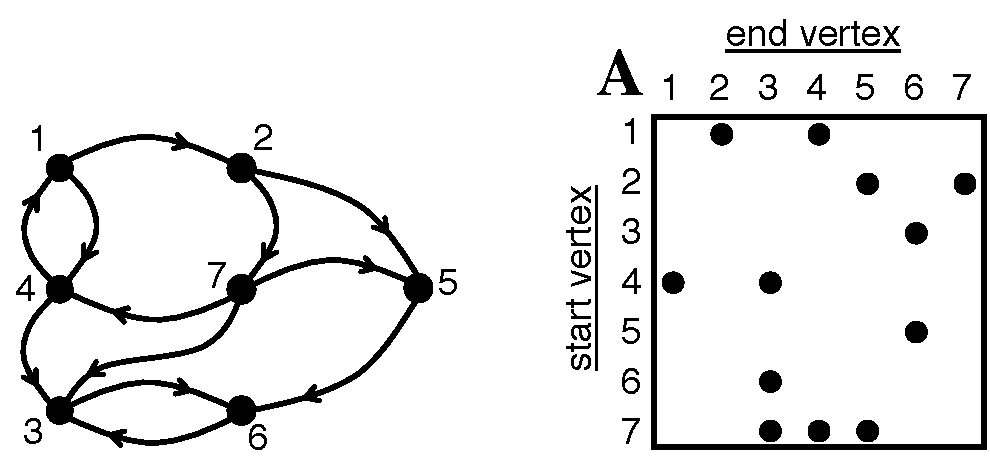
\includegraphics[width=3in]{figures/AdjacencyMatrix.pdf}
      \caption{(left) Seven vertex graph with 12 edges.  Each vertex is labeled with an integer.  (right)  $7 \times 7$ adjacency matrix $\mathbf{A}$ representation of the graph. $\mathbf{A}$ has 12 non-zero entries corresponding to the edges in the graph.}
      \label{fig:AdjacencyMatrix}
\end{figure}

\subsection{Incidence Matrix: Multi-Graphs, Hyper-Graphs, Multipartite Graphs}
An incidence, or edge matrix $\mathbf{E}$, uses the rows to represent every edge in the graph and the columns represent every vertex.  There are a number of conventions for denoting an edge in an incidence matrix.  One such convention is to set $\mathbf{E}_{\rm start}(i,v_1) = 1$ and $\mathbf{E}_{\rm end}(i,v_2) = 1$ to indicate that edge $i$ is a connection from $v_1$ to $v_2$ (see Figure~\ref{fig:IncidenceMatrix}).  Incidence matrices are useful because they can easily represent multi-graphs, hyper-graphs, and multi-partite graphs.  These complex graphs are difficult to capture with an adjacency matrix.  A multi-graph has multiple edges between the same vertices.  If there was another edge, $j$, from $v_1$ to $v_2$, this can be captured in an incidence matrix by setting $\mathbf{E}_{\rm start}(j,v_1) = 1$ and $\mathbf{E}_{\rm end}(j,v_2) = 1$ (see Figure~\ref{fig:IncidenceMatrixMultiHyper}).  In a hyper-graph, one edge can go between more than two vertices.  For example, to denote edge $i$ has a connection from $v_1$ to $v_2$ and $v_3$ can be accomplished by also setting $\mathbf{E}_{\rm end}(i,v_3) = 1$ (see Figure~\ref{fig:IncidenceMatrixMultiHyper}).  Furthermore, $v_1$, $v_2$, and $v_3$ can be drawn from  different classes of vertices and so $\mathbf{E}$ can be used to represent multi-partite graphs.  Thus, an incidence matrix can be used to represent a graph with any set of the following graph properties: directed, weighted, multi-partite, multi-edge, and/or hyper-edge.

\begin{figure}[!htb]
  \centering
    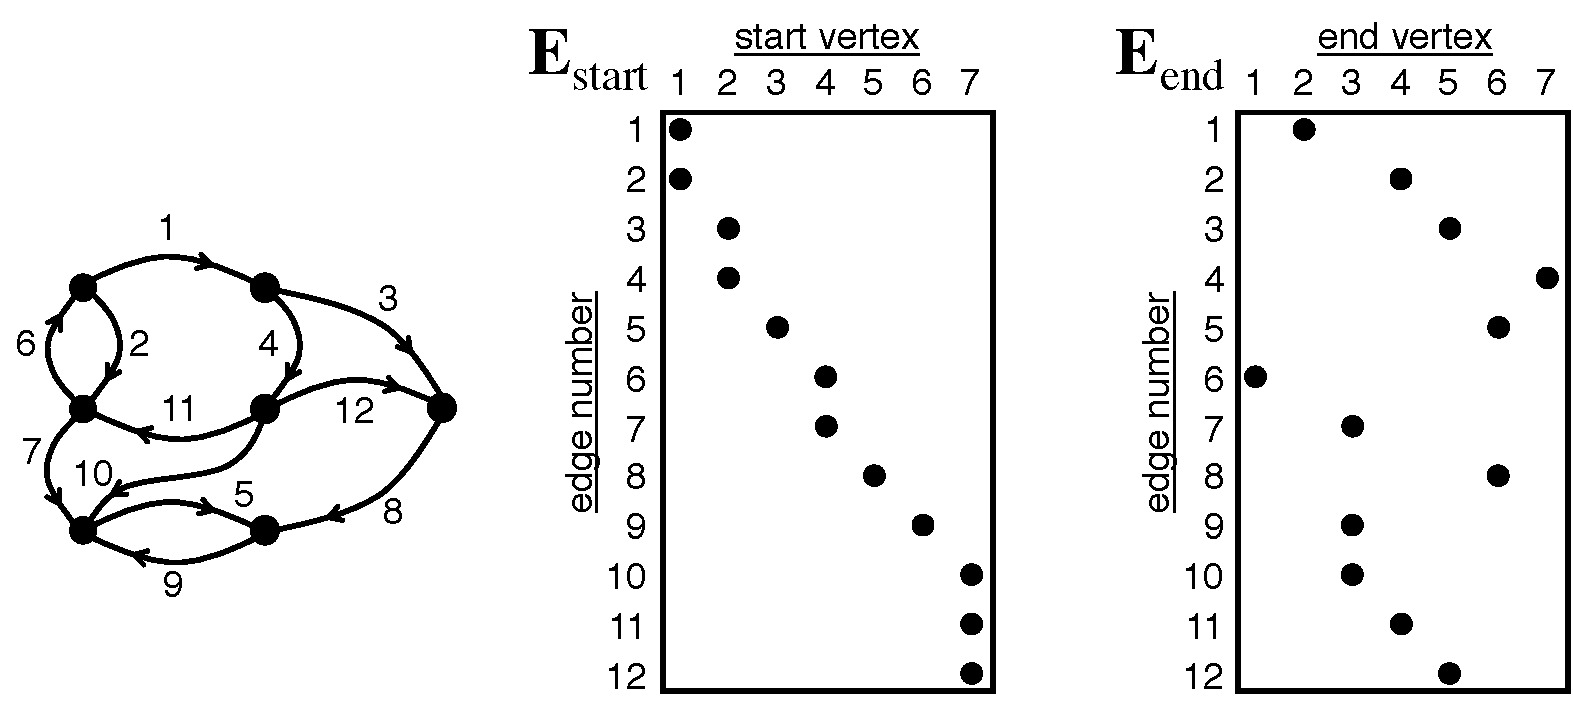
\includegraphics[width=4.5in]{figures/IncidenceMatrix.pdf}
      \caption{(left) Seven vertex graph with 12 edges.  Each edge is labeled with an integer; the vertex labels are the same as in Figure~\ref{fig:AdjacencyMatrix}.  (middle)  $12 \times 7$ incidence matrix $\mathbf{E}_{\rm start}$ representing the starting vertices of the graph edges.   (right)  $12 \times 7$ incidence matrix $\mathbf{E}_{\rm end}$ representing of the ending vertices of the graph edges. Both $\mathbf{E}_{s\rm tart}$ and $\mathbf{E}_{\rm end}$ have 12 non-zero entries corresponding to the edges in the graph.}
      \label{fig:IncidenceMatrix}
\end{figure}
\begin{figure}[!htb]
  \centering
    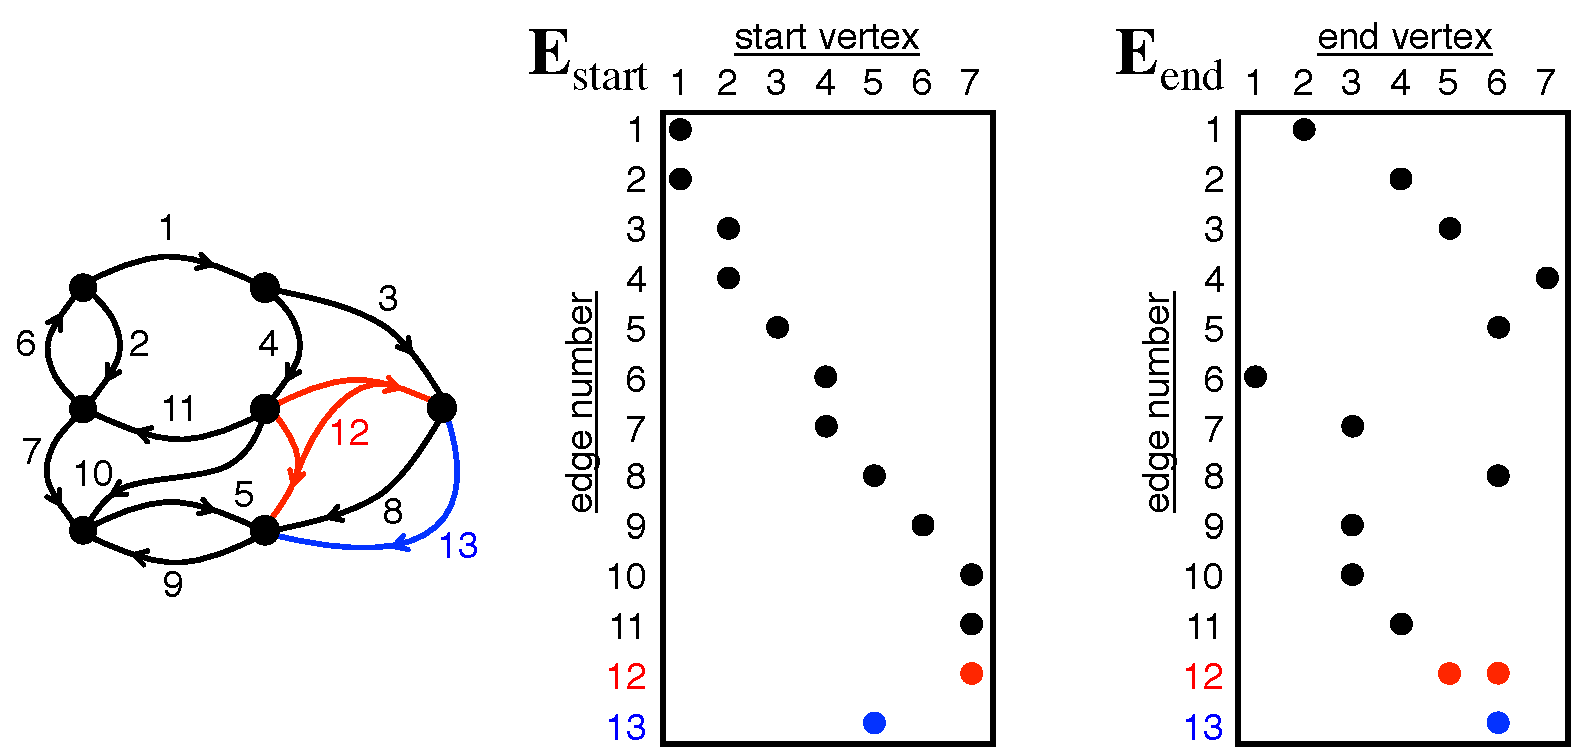
\includegraphics[width=4.5in]{figures/IncidenceMatrixMultiHyper.pdf}
      \caption{Graph and incidence matrices from Figure~\ref{fig:IncidenceMatrix} with a hyper-edge (edge 12) and a multi-edge (edge 13).  The graph is a hyper-graph because edge 12 has more than one end vertex.  The graph is a multi-graph because edge 8 and edge 13 have the same start and end vertex.}
      \label{fig:IncidenceMatrixMultiHyper}
\end{figure}

\section{Matrix Definition: Starting Vertices, Ending Vertices, Edge Weight Types}
  The canonical matrix of the GraphBLAS has $m$ rows and $n$ columns of real numbers.  Such a matrix can be denoted as
$$
  \mathbf{A}: \mathbb{R}^{m \times n}
$$
The canonical row and and column indexes of the matrix $\mathbf{A}$ are $i \in I = \{1,\ldots,m\}$ and $j \in J = \{1,\ldots,n\}$, so that any particular value $\mathbf{A}$ can be denoted as $\mathbf{A}(i,j)$.  [Note: a specific GraphBLAS \emph{implementation} might use IEEE 64 bit double precision floating point numbers to represent real numbers, 64 bit unsigned integers to represent row and column indices, and the compressed sparse rows (CSR) format or the compressed sparse columns (CSC) format to store the non-zero values inside the matrix.]

  A matrix of complex numbers is denoted
$$
  \mathbf{A}: \mathbb{C}^{m \times n}
$$
  A matrix of integers $\{\ldots, -1, 0, 1, \ldots\}$ is denoted
$$
  \mathbf{A}: \mathbb{Z}^{m \times n}
$$
  A matrix of natural numbers $\{1, 2, 3, \ldots\}$ is denoted
$$
  \mathbf{A}: \mathbb{N}^{m \times n}
$$

  Canonical row and column indices are natural numbers $I,J : \mathbb{N}$.  In some GraphBLAS implementations these indices could be non-negative integers  $I = \{0,\ldots,m-1\}$ and $J = \{0,\ldots,n-1\}$.
  
  For the GraphBLAS a matrix is defined as the following 2D mapping
$$
  \mathbf{A} : I \times J \rightarrow \mathbb{S}
$$
where the indices $I, J : \mathbb{Z}$ are finite sets of integers with $m$ and $n$ elements respectively, and  $\mathbb{S} \in \{\mathbb{R},\mathbb{Z},\mathbb{N}, \ldots \}$ is a set of scalars.  Without loss of generality matrices can be denoted
$$
  \mathbf{A}: \mathbb{S}^{m \times n}
$$

If the internal storage format of the matrix needs to be indicated, this can be done by
$$
  \mathbf{A}: \mathbb{S}^{m \times n}_{\rm CSC}  ~~~~~~~~ {\rm or}  ~~~~~~~~ 
  \mathbf{A}: \mathbb{S}^{m \times n}_{\rm CSR}
$$

  A matrix where $m=1$ is a column vector and is denoted
$$
 \mathbf{v} = \mathbb{S}^{m \times 1}
$$
  A matrix where $n=1$ is a row vector and is denoted
$$
  \mathbf{v} = \mathbb{S}^{1 \times n}
$$
  A pure vector is simply denoted
$$
 \mathbf{v} = \mathbb{S}^{m}
$$
whether pure vector it is treated as a column vector or a row vector is determined by its context.

  A scalar is a single element of a set $s \in \mathbb{S}$ and has no matrix dimensions.
%However, in certain implementation contexts it can sometimes be convenient to allow a single element vector/matrix $s : \mathbb{S}^{1 \times 1}$ to have scalar properties.

\section{Scalar Operations: Combining and Scaling Graph Edge Weights}
  The GraphBLAS matrix operations are built on top of scalar operations.  The primary scalar operations are standard arithmetic addition (e.g., $1 + 1 = 2$) and multiplication (e.g., $2 \times 2 = 4$).  The GraphBLAS also allow these scalar operations of addition and multiplication to be defined by the implementation or the user.  To prevent confusion with standard addition and multiplication, $\oplus$ will be used to denote scalar addition and $\otimes$ will be used to denote scalar multiplication.  In this notation, standard arithmetic addition and arithmetic multiplication of real numbers $a, b, c \in \mathbb{R}$, where $\oplus \equiv +$ and $\otimes \equiv \times$ results in
$$
   c = a \oplus b  ~~~~~~~~~ \Rightarrow ~~~~~~~~~ c = a + b
$$
and
$$
   c = a \otimes b  ~~~~~~~~~ \Rightarrow ~~~~~~~~~ c = a \times b
$$
Allowing $\oplus$ and $\otimes$ to be implementation (or user) defined functions enables the GraphBLAS to succinctly implement a wide range of algorithms on scalars of all different types (not just real numbers).

\section{Scalar Properties: Composable Graph Edge Weight Operations}
  Certain $\oplus$ and $\otimes$ combinations  over certain sets of scalars are particular useful because they preserve desirable mathematical properties such as
 %commutativity
%$$
% a \oplus b = b \oplus a ~~~~~~~~~ ~~~~~~~~~ a \otimes b = b \otimes a
%$$
associativity
$$
 (a \oplus b) \oplus c = a \oplus (b \oplus c) ~~~~~~~~~ ~~~~~~~~~ (a \otimes b) \otimes c = a \otimes (b \otimes c)
$$
and distributivity
$$
 a \otimes (b \oplus c)  = (a \otimes b) \oplus (a \otimes c)
$$

%  In most cases, if these properties are true for scalar operations they will also be true for their corresponding matrix operations.  
Associativity, and distributivity are \emph{extremely} useful properties for building graph applications because they allow the builder to swap operations without changing the result. They also increase opportunities for exploiting parallelism by the runtime. 

  Example combinations of $\oplus$ and $\otimes$ that preserve scalar associativity and distributivity include (but are not limited to) standard arithmetic
$$
  \oplus \equiv + ~~~~~~~~~ \otimes \equiv \times ~~~~~~~~~ a, b, c \in \mathbb{R}
$$
max-plus algebras
$$
  \oplus \equiv \max ~~~~~~~~~ \otimes \equiv + ~~~~~~~~~ a, b, c \in \{-\infty \cup \mathbb{R}\}
$$
max-min algebras
$$
  \oplus \equiv \max ~~~~~~~~~ \otimes \equiv \min ~~~~~~~~~ a, b, c \in [0,\infty]
$$
finite (Galois) fields such as GF(2)
$$
  \oplus \equiv {\rm xor} ~~~~~~~~~ \otimes \equiv {\rm and} ~~~~~~~~~ a, b, c \in [0,1]
$$
and power set algebras
$$
  \oplus \equiv \cup ~~~~~~~~~ \otimes \equiv \cap ~~~~~~~~~ a, b, c \subset \mathbb{Z}
$$

These operations also preserve scalar commutativity. Other functions can also be defined for $\oplus$ and $\otimes$ that do not preserve the above properties.  For example, it is often useful for $\oplus$ or $\otimes$ to pull in other data such as vertex labels of a graph, such as the select2nd operation used in breadth-first search. 

\section{Matrix Properties: Composable Operations on Entire Graphs}
  Associativity, distributivity, and commutativity are very powerful properties of the GraphBLAS and separate it from standard graph libraries because these properties allow the GraphBLAS to be composable (i.e., you can re-order operations and know that you will get the same answer).  Composability is what allows the GraphBLAS to implement a wide range of graph algorithms with just a few functions.

  Let $\mathbf{A}, \mathbf{B}, \mathbf{C} \in \mathbb{S}^{m \times n}$, be matrices with elements $a = \mathbf{A}(i,j)$, $b = \mathbf{B}(i,j)$, and $c = \mathbf{C}(i,j)$.  Associativity, distributivity, and commutativity of scalar operations translates into similar properties on matrix operations in the following manner.

\begin{description}
\item[Additive Commutativity] Allows graphs to be swapped and combined via matrix element-wise addition (see Figure~\ref{fig:AdjacencyMatrixAdd}) without changing the result
  $$
      a \oplus b = b \oplus a  ~~~~~~~~~ \Rightarrow ~~~~~~~~~
      \mathbf{A} \oplus \mathbf{B} = \mathbf{B} \oplus \mathbf{A}
  $$
  where matrix element-wise addition is given by
     $\mathbf{C}(i,j) = \mathbf{A}(i,j) \oplus \mathbf{B}(i,j)$
     
\item[Multiplicative Commutativity] Allows graphs to be swapped, intersected, and scaled via matrix element-wise multiplication (see Figure~\ref{fig:AdjacencyMult}) without changing the result
  $$
      a \otimes b = b \otimes a  ~~~~~~~~~ \Rightarrow ~~~~~~~~~
      \mathbf{A} \otimes \mathbf{B} = \mathbf{B} \otimes \mathbf{A}
  $$
    where matrix element-wise (Hadamard) multiplication is given by
     $\mathbf{C}(i,j) = \mathbf{A}(i,j) \otimes \mathbf{B}(i,j)$

\item[Additive Associativity] Allows graphs to be combined via matrix element-wise addition in any grouping without changing the result
  $$
      (a \oplus b) \oplus c = a \oplus (b \oplus c)   ~~~~~~~~~ \Rightarrow ~~~~~~~~~
      (\mathbf{A} \oplus \mathbf{B}) \oplus \mathbf{C} = \mathbf{A} \oplus (\mathbf{B} \oplus \mathbf{C})
  $$

\item[Multiplicative Associativity] Allows graphs to be intersected and scaled via matrix element-wise multiplication in any grouping without changing the result
  $$
      (a \otimes b) \otimes c = a \otimes (b \otimes c)   ~~~~~~~~~ \Rightarrow ~~~~~~~~~
      (\mathbf{A} \otimes \mathbf{B}) \otimes \mathbf{C} = \mathbf{A} \otimes (\mathbf{B} \otimes \mathbf{C})
  $$

\item[Element-Wise Distributivity] Allows graphs to be intersected and/or scaled and then combined or vice-verse without changing the result
  $$
      a \otimes (b \oplus c) = (a \otimes b) \oplus (a \otimes c)   ~~~~~~~~~ \Rightarrow ~~~~~~~~~
      \mathbf{A} \otimes (\mathbf{B} \oplus \mathbf{C}) = (\mathbf{A} \otimes \mathbf{B}) \oplus (\mathbf{A} \otimes \mathbf{C})
  $$

\item[Matrix Multiply Distributivity] Allows graphs to be transformed via matrix multiply and then combined or vice-verse without changing the result
  $$
      a \otimes (b \oplus c) = (a \otimes b) \oplus (a \otimes c)   ~~~~~~~~~ \Rightarrow ~~~~~~~~~
      \mathbf{A} (\mathbf{B} \oplus \mathbf{C}) = (\mathbf{A} \mathbf{B}) \oplus (\mathbf{A} \mathbf{C})
  $$
  where matrix multiply $\mathbf{C} = \mathbf{A} \mathbf{B}$ is given by
  $$
   {\bf C}(i,j) = \bigoplus_{k=1}^l {\bf A}(i,k) \otimes {\bf B}(k,j)
  $$
  for matrices  ${\bf A}: \mathbb{S}^{m \times l}$,  ${\bf B}: \mathbb{S}^{l \times n}$, and ${\bf C}: \mathbb{S}^{m \times n}$

\item[Matrix Multiply Associativity] is another implication of scalar distributivity and allows graphs to be transformed via matrix multiply in any grouping without changing the result
  $$
      a \otimes (b \oplus c) = (a \otimes b) \oplus (a \otimes c)   ~~~~~~~~~ \Rightarrow ~~~~~~~~~
      (\mathbf{A} \mathbf{B}) \mathbf{C} = \mathbf{A} (\mathbf{B} \mathbf{C})
  $$
\item[Matrix Multiply Commutativity] In general, $\mathbf{A} \mathbf{B} \neq \mathbf{B} \mathbf{A}$.  Some cases where $\mathbf{A} \mathbf{B} = \mathbf{B} \mathbf{A}$ include when one matrix is all zeros, one matrix is the identity matrix, both matrices are diagonal matrices, or both matrices are rotation matrices.
\end{description}

\begin{figure}[htb]
  \centering
    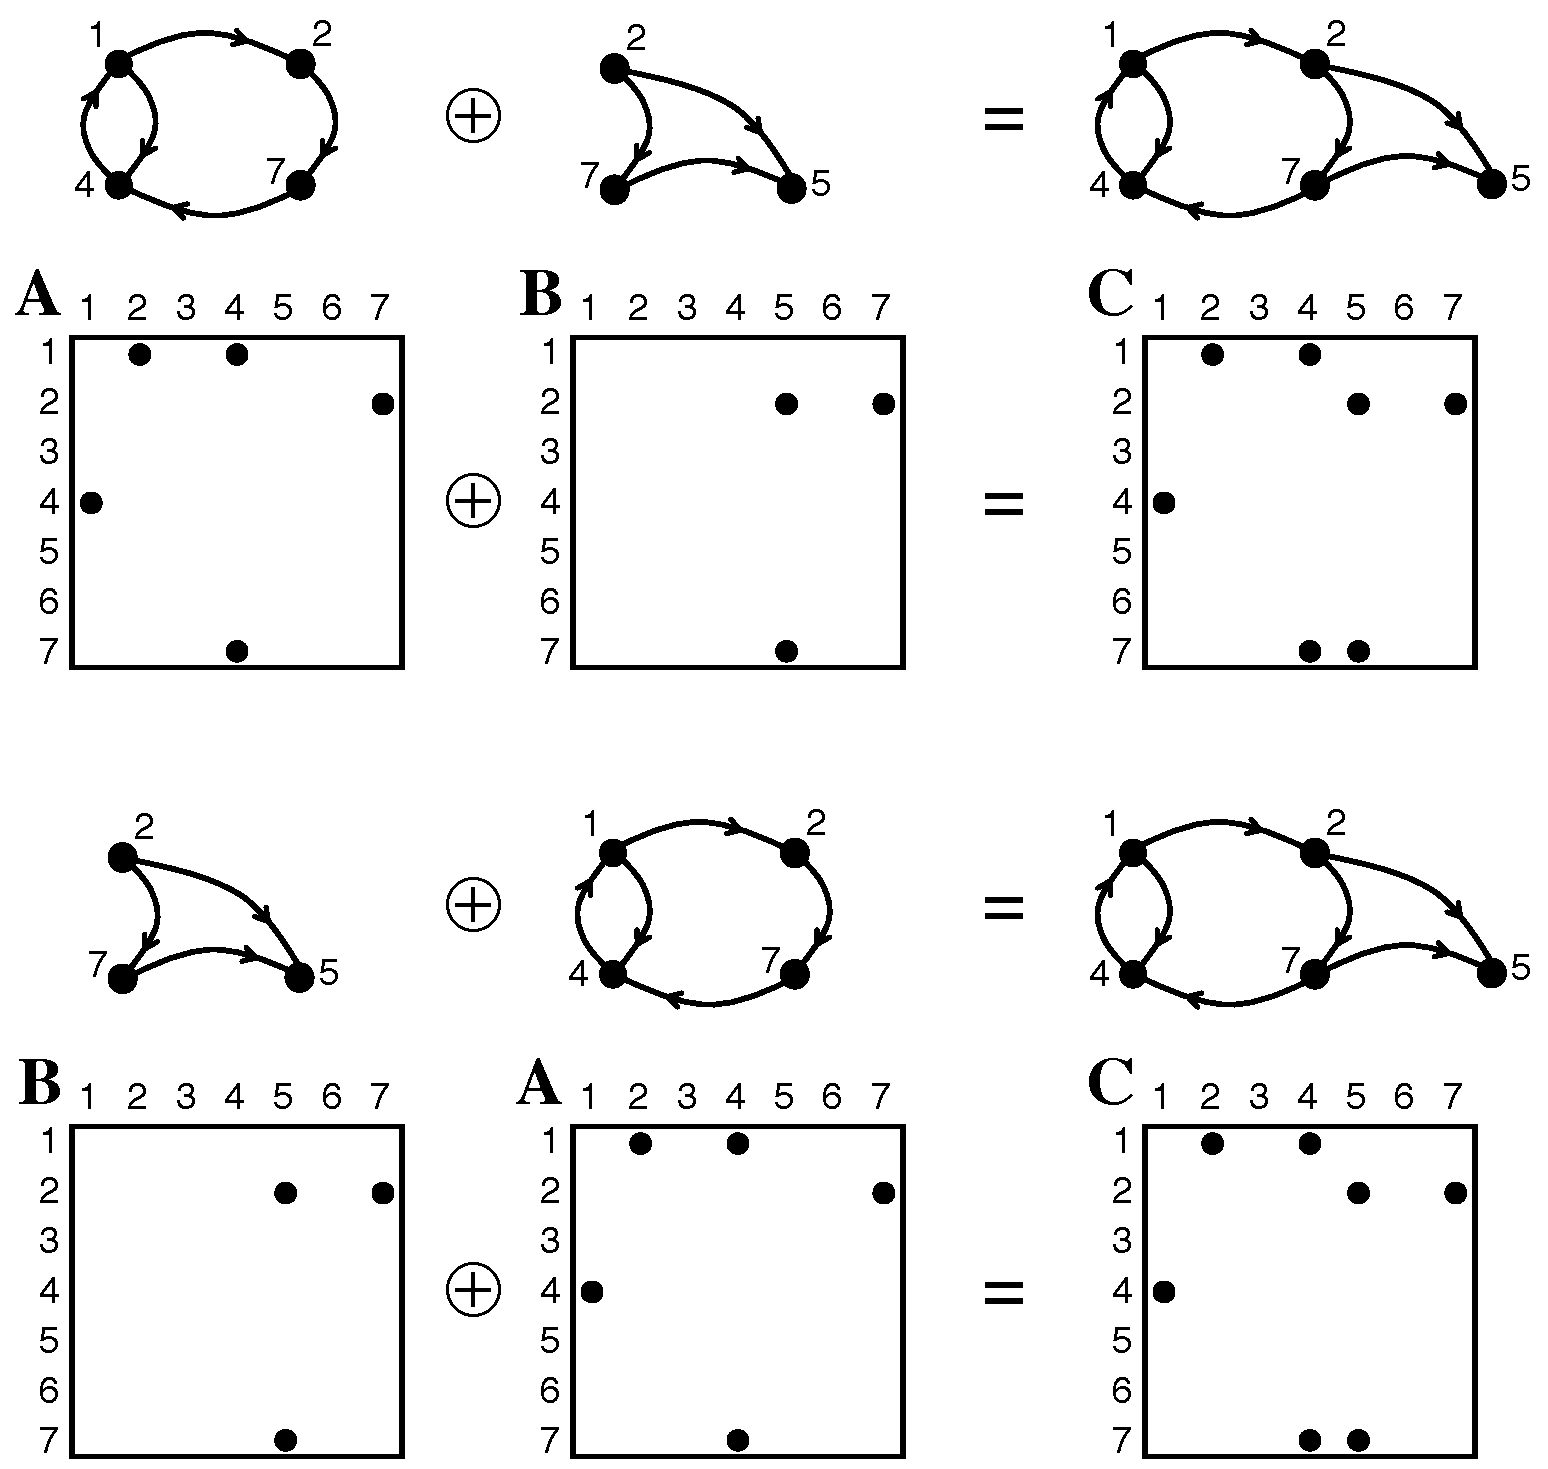
\includegraphics[width=3in]{figures/AdjacencyMatrixAdd.pdf}
      \caption{Illustration of the commutative property of the element-wise addition of two graphs and their corresponding adjacency matrix representations.}
      \label{fig:AdjacencyMatrixAdd}
\end{figure}
\begin{figure}[!htb]
  \centering
    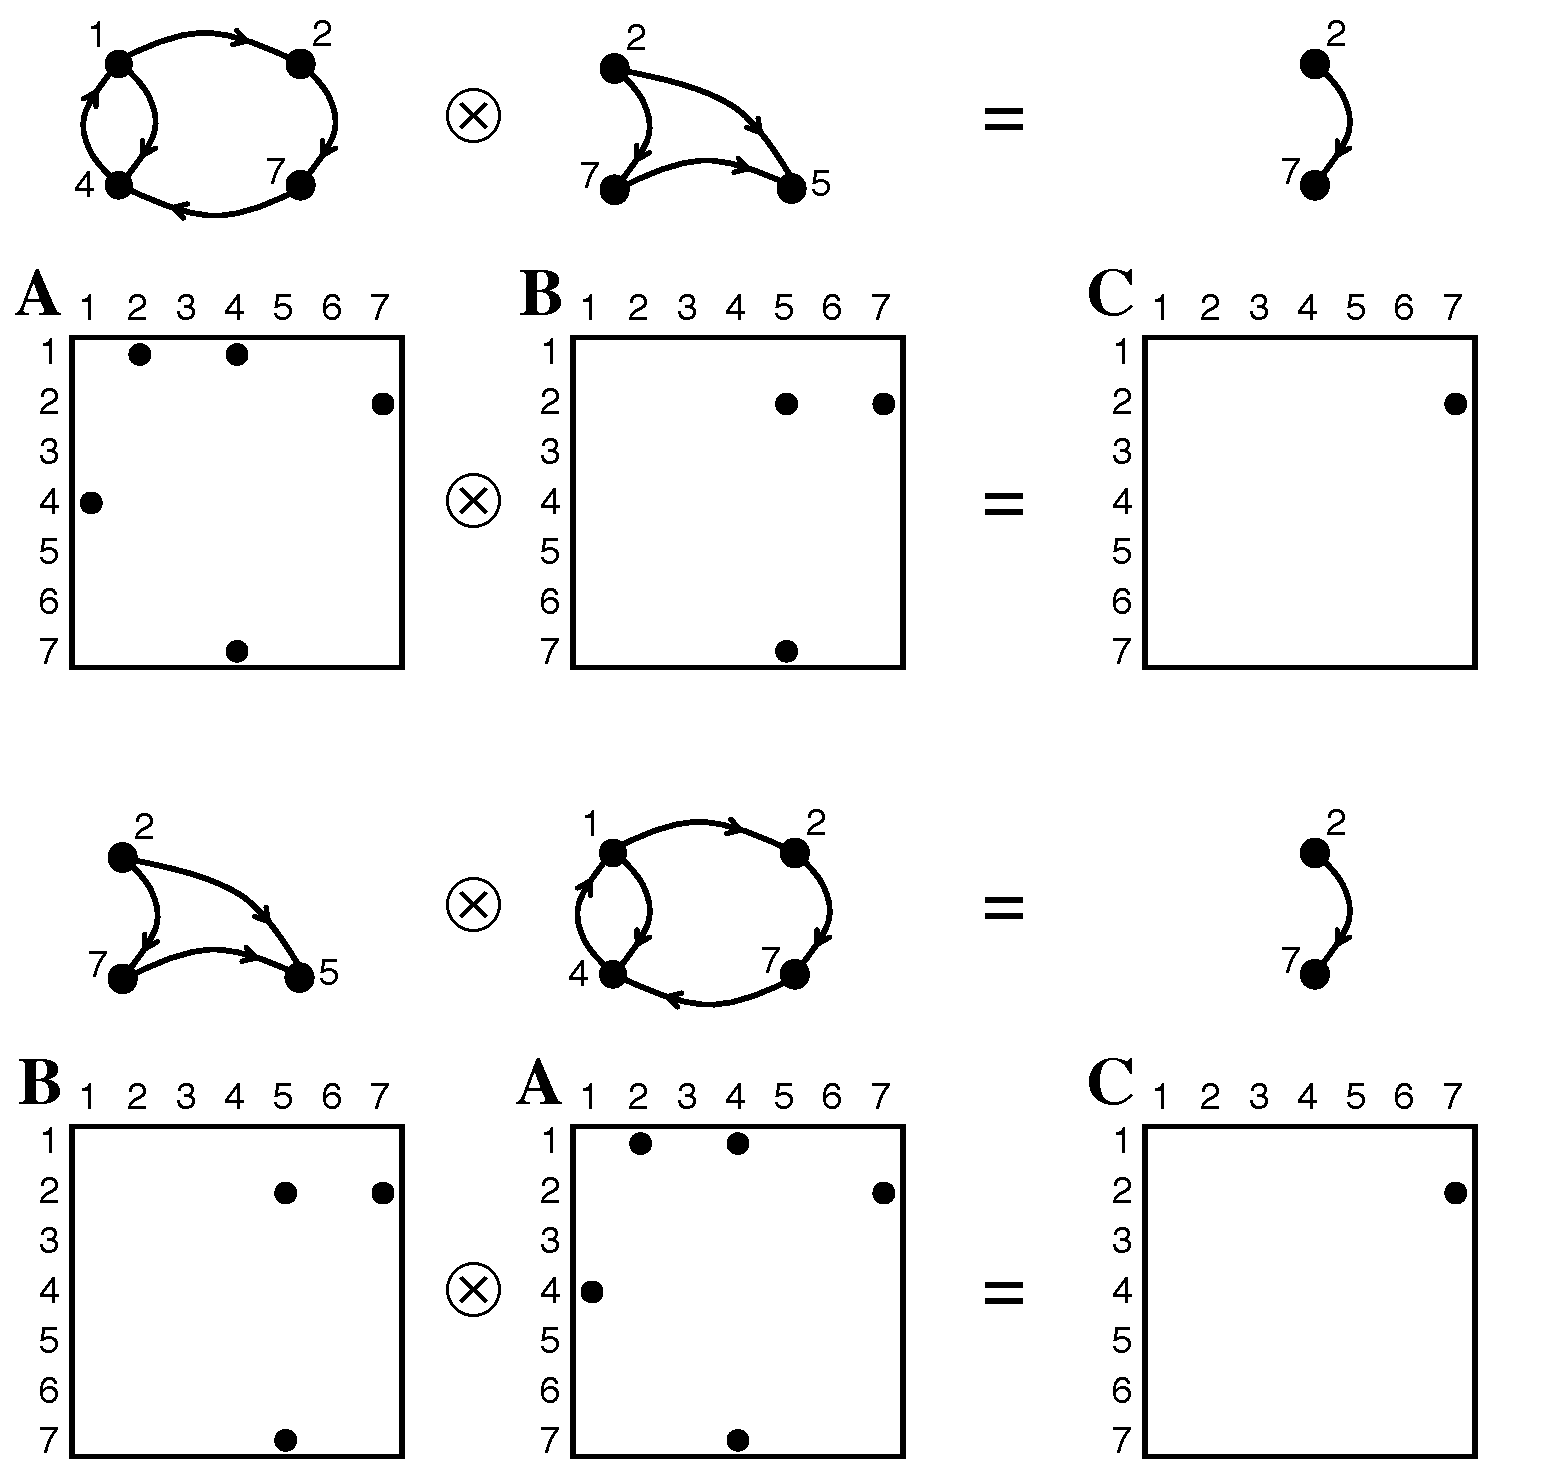
\includegraphics[width=3in]{figures/AdjacencyMatrixMult.pdf}
      \caption{Illustration of the commutative property of the element-wise multiplication of two graphs and their corresponding adjacency matrix representations.}
      \label{fig:AdjacencyMatrixMult}
\end{figure}


\section{0-Element: No Graph Edge}
  Sparse matrices play an important role in GraphBLAS.  Many implementations of sparse matrices reduce storage by not storing the 0 valued elements in the matrix.  In adjacency matrices, the 0 element is equivalent to no edge from the vertex represented by row to the vertex represented by the column. In incidence matrices, the 0 element is equivalent to the edge represented by row not including the vertex represented by the column.  In most cases, the 0 element is standard arithmetic 0.  The GraphBLAS also allows the 0 element to be defined by the implementation or user.  This can be particularly helpful when combined with user defined $\oplus$ and $\otimes$ operations.  Specifically, if the 0 element has certain properties with respect scalar $\oplus$ and $\otimes$, then sparsity of matrix operations can be managed efficiently.  These properties are the additive identity
$$
     a \oplus 0 = a
$$
and the multiplicative annihilator
$$
     a \otimes 0 = 0
$$
Note: the above behavior of $\oplus$ and $\otimes$ with respect to 0 is a requirement for the GraphBLAS.

  Example combinations of $\oplus$ and $\otimes$ that exhibit the additive identity and multiplicative annihilator are:

%Standard arithmetic over the real numbers $a \in \mathbb{R}$, 
%$\oplus \equiv +$, $\otimes \equiv \times$, $0 \equiv 0$ $\Rightarrow$ \\
%additive identity: $a \oplus 0  =  a + 0 = a$ \\
%multiplicative annihilator: $a \otimes 0 = a \times 0 = 0$
%
%Max-plus algebras over $a \in \{-\infty \cup \mathbb{R}\}$, $\oplus \equiv \max$, $\otimes \equiv +$, $0 \equiv -\infty$ $\Rightarrow$ \\
%additive identity: $a \oplus 0  =  \max(a,-\infty) = a$ \\
%multiplicative annihilator: $a \otimes 0 = a + -\infty = -\infty$
%
%Min-max algebras over $a \in [0,\infty]$, $\oplus \equiv \min$, $\otimes \equiv \max$, $0 \equiv \infty$ $\Rightarrow$ \\
%additive identity: $a \oplus 0  =  \min(a,\infty) = a$ \\
%multiplicative annihilator: $a \otimes 0 = \max(a,\infty) = \infty$
%
%The Galois field GF(2) over $a \in [0,1]$, $\oplus \equiv {\rm xor}$, $\otimes \equiv {\rm and}$, $0 \equiv 0$ $\Rightarrow$ \\
%additive identity: $a \oplus 0  = {\rm xor}(a,0) = a$ \\
%multiplicative annihilator: $a \otimes 0 = {\rm and}(a,0) = 0$
%
%Power set algebras over sets of integers $a \subset \mathbb{Z}$, $\oplus \equiv \cup$, $\otimes \equiv \cap$, $0 \equiv \emptyset$ $\Rightarrow$ \\
%additive identity: $a \oplus 0  =  a \cup \emptyset = a$ \\
%multiplicative annihilator: $a \otimes 0 = a \cap \emptyset = \emptyset$

\begin{description}

\item[Arithmetic on Real Numbers (${+}.{\times}$)] Given standard arithmetic over the real numbers
$$
  a \in \mathbb{R}
$$
where addition is
$$
  \oplus \equiv +
$$
multiplication is
$$
  \otimes \equiv \times
$$
and zero is
$$
  0 \equiv 0
$$
which results in additive identity
$$
  a \oplus 0  =  a + 0 = a
$$
and multiplicative annihilator
$$
  a \otimes 0 = a \times 0 = 0
$$

\index{max-plus algebra}\item[Max-Plus Algebra (${\max}.{+}$)] Given real numbers with a minimal element
$$
  a \in \{\text{-}\infty \cup \mathbb{R}\}
$$
where addition is
$$
  \oplus \equiv \max
$$
multiplication is
$$
  \otimes \equiv +
$$
and zero is
$$
  0 \equiv \text{-}\infty
$$
which results in additive identity
$$
  a \oplus 0  =  \max(a,\text{-}\infty) = a
$$
and multiplicative annihilator
$$
  a \otimes 0 = a + \text{-}\infty = \text{-}\infty
$$

\index{min-plus algebra}\item[Min-Plus Algebra (${\min}.{+}$)] Given real numbers with a maximal element
$$
  a \in \{\mathbb{R} \cup \infty\}
$$
where addition is
$$
  \oplus \equiv \min
$$
multiplication is
$$
  \otimes \equiv +
$$
and zero is
$$
  0 \equiv \infty
$$
which results in additive identity
$$
  a \oplus 0  =  \min(a,\infty) = a
$$
and multiplicative annihilator
$$
  a \otimes 0 = a + \infty = \infty
$$


\index{max-min algebra}\item[Max-Min Algebra (${\max}.{\min}$)] Given non-negative real numbers
$$
  \mathbb{R}_{\geq 0} = \{a : 0 \leq a < \infty\}
$$
where addition is
$$
  \oplus \equiv \max
$$
multiplication is
$$
  \otimes \equiv \min
$$
and zero is
$$
  0 \equiv 0
$$
which results in additive identity
$$
  a \oplus 0  =  \max(a,0) = a
$$
and multiplicative annihilator
$$
  a \otimes 0 = \min(a,0) = 0
$$

\index{min-max algebra}\item[Min-Max Algebra (${\min}.{\max}$)] Given non-positive real numbers
$$
  \mathbb{R}_{\leq 0} = \{a : \text{-}\infty < a \leq 0\}
$$
where addition is
$$
  \oplus \equiv \min
$$
multiplication is
$$
  \otimes \equiv \max
$$
and zero is
$$
  0 \equiv 0
$$
which results in additive identity
$$
  a \oplus 0  =  \min(a,0) = a
$$
and multiplicative annihilator
$$
  a \otimes 0 = \max(a,0) = 0
$$

\index{Galois field}\index{GF(2)}\item[Galois Field (${{\rm xor}}.{{\rm and}}$)] Given a set of two numbers
$$
  a \in \{0,1\}
$$
where addition is
$$
  \oplus \equiv \text{xor}
$$
multiplication is
$$
  \otimes \equiv \text{and}
$$
and zero is
$$
  0 \equiv 0
$$
which results in additive identity
$$
  a \oplus 0  =  \text{xor}(a,0) = a
$$
and multiplicative annihilator
$$
  a \otimes 0 = \text{and}(a,0) = 0
$$

\index{power set}\item[Power Set (${\cup}.{\cap}$)] Given any subset of integers
$$
  a \subset \mathbb{Z}
$$
where addition is
$$
  \oplus \equiv \cup
$$
multiplication is
$$
  \otimes \equiv \cap
$$
and zero is
$$
  0 \equiv \emptyset
$$
which results in additive identity
$$
  a \oplus 0  =   a \cup \emptyset = a
$$
and multiplicative annihilator
$$
  a \otimes 0 = a \cap \emptyset = \emptyset
$$
\end{description}

The above examples are a small selection of the operators and sets that are useful for building graph algorithms.  Many more are possible.  The ability to change the  scalar values and operators while preserving the overall behavior of the graph operations is one of the principal benefits of using matrices for graph algorithms.  For example, relaxing the requirement that the multiplicative annihilator be the additive identity, as in the above examples, yields additional operations, such as

\begin{description}
\index{max-max algebra}\item[Max-Max Algebra (${\max}.{\max}$)] Given non-positive real numbers with a minimal element
$$
  a \in \{\text{-}\infty \cup \mathbb{R}_{\leq 0} \}
$$
where addition is
$$
  \oplus \equiv \max
$$
multiplication is (also)
$$
  \otimes \equiv \max
$$
and zero is
$$
  0 \equiv \text{-}\infty
$$
which results in additive identity
$$
  a \oplus 0  =  \max(a,\text{-}\infty) = a
$$

\index{min-min algebra}\item[Min-Min Algebra (${\min}.{\max}$)] Given non-negative real numbers with a maximal element
$$
  a \in \{\mathbb{R}_{\geq 0} \cup \infty\}
$$
where addition is
$$
  \oplus \equiv \min
$$
multiplication is (also) 
$$
  \otimes \equiv \min
$$
and zero is
$$
  0 \equiv \infty
$$
which results in additive identity
$$
  a \oplus 0  =  \min(a,\infty) = a
$$
\end{description}

\section{Matrix Graph Operations Overview}

The core of the GraphBLAS is the ability to perform a wide range of graph operations on diverse types of graphs with a small number of matrix operations:
\begin{description}
\item[Matrix\_build] {\bf build} a sparse {\bf Matrix} from row, column, and value tuples.  Example graph operations include: graph construction from a set of starting vertices, ending vertices, and edge weights.
\item[Vector\_build] {\bf build} a sparse {\bf Vector} from index value tuples.
\item[Matrix\_extractTuples] {\bf extract} the row, column, and value {\bf Tuples} corresponding to the non-zero elements in a sparse {\bf Matrix}.  Example graph operations include: extracting a graph from is matrix represent.
\item[Vector\_extractTuples] {\bf extract} the index and value {\bf Tuples} corresponding to the non-zero elements in a sparse {\bf vector}.
\item[transpose] Flips or {\bf transpose}s the rows and the columns of a sparse matrix.  Implements reversing the direction of the graph.  Can be implemented with  {\bf ExtracTuples} and {\bf BuildMatrix}.
\item[mxm, mxv, vxm] {\bf m}atrix {\bf x} (times) {\bf m}atrix,  {\bf m}atrix {\bf x} (times) {\bf v}ector, {\bf v}ector {\bf x} (times) {\bf m}atrix.   Example graph operations include: single-source breadth first search, multi-source breadth first search, weighted breadth first search.
\item[extract] {\bf extract} sub-matrix from a larger matrix. Example graph operations include: sub-graph selection.  Can be implemented with {\bf Matrix\_build} and {\bf mxm} or {\bf Vector\_build} and {\bf mxv} or {\bf vxm}.
\item[assign] {\bf assign} matrix or vector to a set of indices in a larger matrix or vector.  Example graph operations include: sub-graph assignment.  Can be implemented with {\bf Matrix\_build} and {\bf mxm} or {\bf Vector\_build} and {\bf mxv} or {\bf vxm}.
\item[eWiseAdd, eWiseMult] {\bf e}lement{\bf Wise} {\bf Add}ition of matrices or vectors, {\bf e}lement{\bf Wise} {\bf Mult}iplication (Hadamard product) of matrices  or vectors. Example graph operations include: graph union and intersection along with edge weight scale and combine.
\item[apply] {\bf apply} unary function to a matrix or a vector.  Example graph operations include: graph edge weight modification.  Can be implemented via {\bf eWiseAdd} or {\bf eWiseMult}.
\item[reduce] {\bf reduce} sparse matrix.  Implements vertex degree calculations.  Can be implemented via {\bf mxm}, {\bf mxv}, or {\bf vxm}.
\end{description}
The above set of functions has been shown to be useful for implementing a wide range of graph algorithms.  These functions strike a balance between providing enough functions to be useful to an application builders and while being few enough that they can be implemented effectively.  Furthermore, from an implementation perspective, there are only six functions that are truly fundamental: {\bf Matrix\_build}, {\bf Matrix\_extractTuples}, {\bf transpose}, {\bf mxm},  {\bf eWiseAdd} and {\bf eWiseMult}.  The other GraphBLAS functions can be implemented from these six functions.


\section{Matrix\_build: Edge List to Graph}
  The GraphBLAS may use a variety of internal formats for representing sparse matrices.  This data can often be imported as triples of vectors ${\bf i}$, ${\bf j}$, and ${\bf v}$ corresponding to the non-zero elements in the sparse matrix.  Constructing an $m \times n$ sparse matrix from triples can be denoted
$$
   \mathbf{C}  ~~ {\textcolor{blue}{\oplus}}{=} ~~  \mathbb{S}^{m \times n}({\bf i},{\bf j},{\bf v},{\textcolor{blue}{\oplus}})
$$
where ${\bf i} : I^L$, ${\bf j}: J^L$, ${\bf i}, {\bf v}: \mathbb{S}^L$, are all $L$ element vectors, and the symbols in \textcolor{blue}{blue} represent optional operations that can be specified by the user.  The optional ${\textcolor{blue}{\oplus}}{=}$ denotes the option of adding the product to the existing values in ${\bf C}$.  The optional  ${\textcolor{blue}{\oplus}}$ function defines how multiple entries with the same row and column are handled.  If ${\textcolor{blue}{\oplus}}$ is undefined then the default is to combine the values using standard arithmetic addition $+$.  Other variants include replacing any or all of the vector inputs with single element vectors.  For example
$$
   \mathbf{C} = \mathbb{S}^{m \times n}({\bf i},{\bf j},1)
$$
would use the value of $1$ for input values.  Likewise, a row vector can be constructed using
$$
   \mathbf{C} = \mathbb{S}^{m \times n}(1,{\bf j},{\bf v})
$$
and a column vector can be constructed using
$$
   \mathbf{C} = \mathbb{S}^{m \times n}({\bf i},1,{\bf v})
$$
The value type of the sparse matrix can be further specified via
$$
   \mathbf{C}: \mathbb{R}^{m \times n}({\bf i},{\bf j},{\bf v})
$$

\section{Vector\_build}
  Using notation similar to {\bf Matrix\_build}, constructing an $m$ element abstract sparse vector can be denoted
$$
   \mathbf{c}  ~~ {\textcolor{blue}{\oplus}}{=} ~~  \mathbb{S}^{m}({\bf i},{\bf v},{\textcolor{blue}{\oplus}})
$$
  
\section{Matrix\_extractTuples: Graph to Vertex List}
  It is expected the GraphBLAS will need to send results to other software components.  Triples are a common interchange format.  The GraphBLAS {\bf ExtractTuples} command performs this operation by extracting the non-zero triples from a sparse matrix and can be denoted mathematically as
$$
	({\bf i},{\bf j},{\bf v}) = {\bf A}
$$

\section{Vector\_extractTuples}
  Using notation similar to {\bf Matrix\_extractTuples}, extracting the non-zero elements from a sparse vector and can be denoted mathematically as
$$
	({\bf i},{\bf v}) = {\bf c}
$$

\section{transpose: Swap Start and End Vertices}
  Swapping the rows and columns of a sparse matrix is a common tool for changing the direction of vertices in a graph (see Figure~\ref{fig:AdjacencyMatrixTranspose}).  The transpose is denoted as
$$
     {\bf C} ~~ {\textcolor{blue}{\oplus}}{=} ~~ {\bf A}^{\sf T}
$$   
or more explicitly
$$
     {\bf C}(j,i) = {\bf C}(j,i) ~~ {\textcolor{blue}{\oplus}} ~~ {\bf A}(i,j)
$$   
where ${\bf A}:\mathbb{S}^{m \times n}$ and ${\bf C}:\mathbb{S}^{n \times m}$

Transpose can be implemented using a combination of {\bf Matrix\_build} and {\bf Matrix\_extractTuples} as follows
$$
	({\bf i},{\bf j},{\bf v}) = {\bf A}
$$
$$
   \mathbf{C} = \mathbb{S}^{n \times m}({\bf j},{\bf i},{\bf v})
$$

\begin{figure}[!htb]
  \centering
    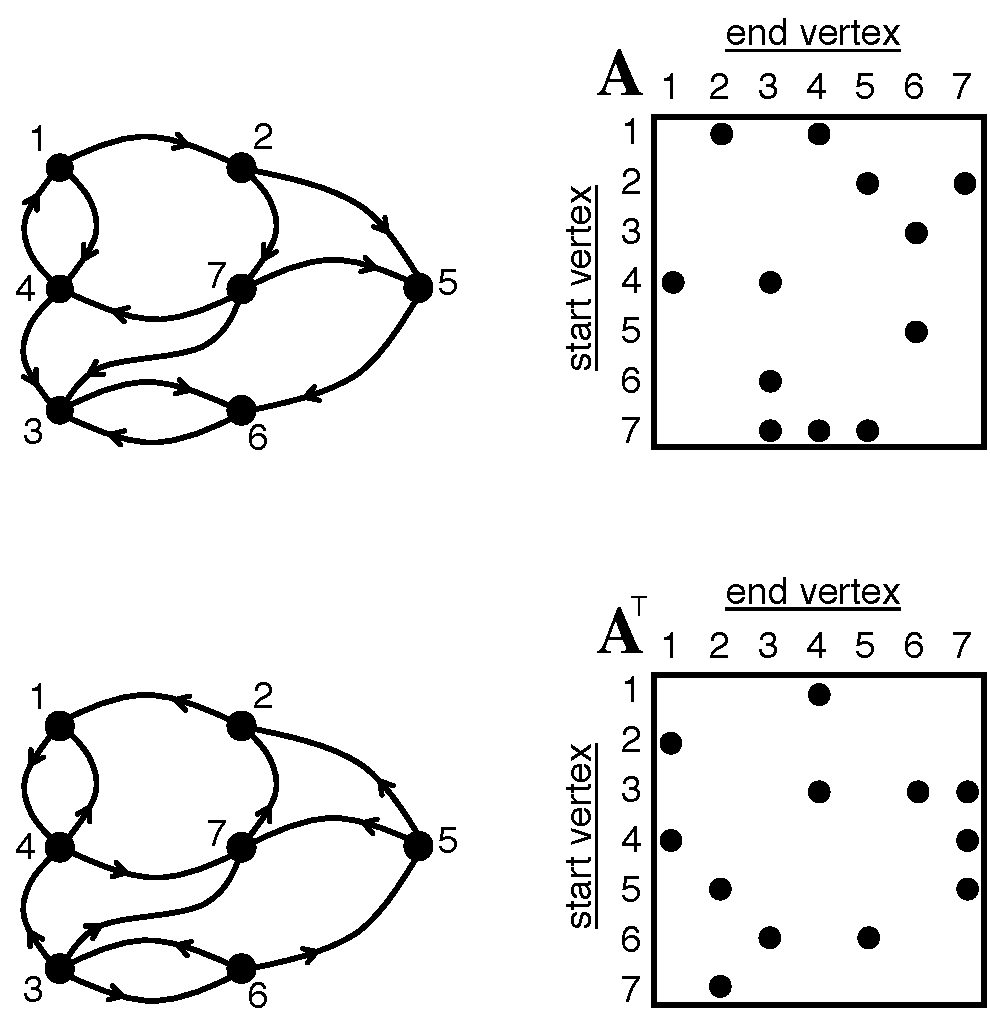
\includegraphics[width=3in]{figures/AdjacencyMatrixTranspose.pdf}
      \caption{Transposing the adjacency matrix of a graph switches the directions of its edges.}
      \label{fig:AdjacencyMatrixTranspose}
\end{figure}
  
\section{mxm: Weighted, Multi-Source, Breadth-First-Search}

Matrix multiply is the most important operation in the GraphBLAS and can be used to implement a wide range of graph algorithms.  Examples include finding the nearest neighbors of a vertex (see Figure~\ref{fig:AdjacencyMatrixBFS}) and constructing an adjacency matrix from an incidence matrix (see Figure~\ref{fig:AdjacencyToIncidence}). In its most common form, {\bf mxm} performs a matrix multiply using standard arithmetic addition and multiplication
$$
   {\bf C} = {\bf A} {\bf B}
$$
or more explicitly
$$
   {\bf C}(i,j) = \sum_{k=1}^l {\bf A}(i,k) {\bf B}(k,j)
$$
where ${\bf A}: \mathbb{R}^{m \times l}$,  ${\bf B}: \mathbb{R}^{l \times n}$, and ${\bf C}: \mathbb{R}^{m \times n}$. {\bf mxm} has many important variants that include accumulating results, transposing inputs or outputs, and user defined addition and multiplication.  These variants can be used alone or in combination.  When these variants are combined with the wide range of graphs that can be represented with sparse matrices, this results in many thousands of distinct graph operations that can be succinctly captured by multiplying two sparse matrices.   As will be described subsequently, all of these variants can be represented by the following mathematical statement
$$
   {\bf C}^{\textcolor{blue}{\sf T}} ~~ {\textcolor{blue}{\oplus}}{=} ~~ {\bf A}^{\textcolor{blue}{\sf T}} ~ {\oplus}.{\otimes} ~ {\bf B}^{\textcolor{blue}{\sf T}}
$$
where  ${\bf A}: \mathbb{S}^{m \times l}$,  ${\bf B}: \mathbb{S}^{l \times m}$, and ${\bf C}: \mathbb{S}^{m \times n}$, ${\textcolor{blue}{\oplus}}{=}$ denotes the option of adding the product to the existing values in ${\bf C}$, and ${\oplus}.{\otimes}$ makes explicit that ${\oplus}$ and ${\otimes}$ can be user defined functions.

%Special cases of {\bf mx,} include
%\begin{itemize}
%\item  {\bf SpMxSpV} : Sparse matrix times sparse vector
%\item  {\bf SpMxV} : Sparse matrix times dense vector
%\item {\bf SpMxM} : Sparse matrix times multiple dense vectors
%\item {\bf SpMxM} : Sparse matrix times dense matrix
%\end{itemize}

\begin{figure}[!htb]
  \centering
    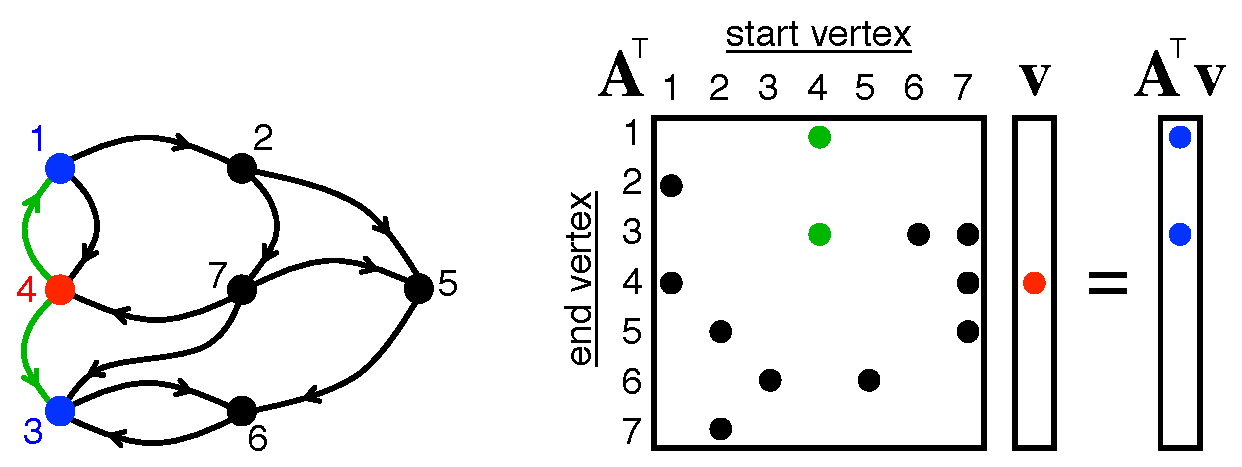
\includegraphics[width=4in]{figures/AdjacencyMatrixBFS.pdf}
      \caption{(left) Breadth-first-search of a graph starting at vertex 4 and traversing out to vertices 1 and 3.  (right) Matrix-vector multiplication of the adjacency matrix of a graph performs the equivalent operation.}
      \label{fig:AdjacencyMatrixBFS}
\end{figure}
\begin{figure}[!htb]
  \centering
    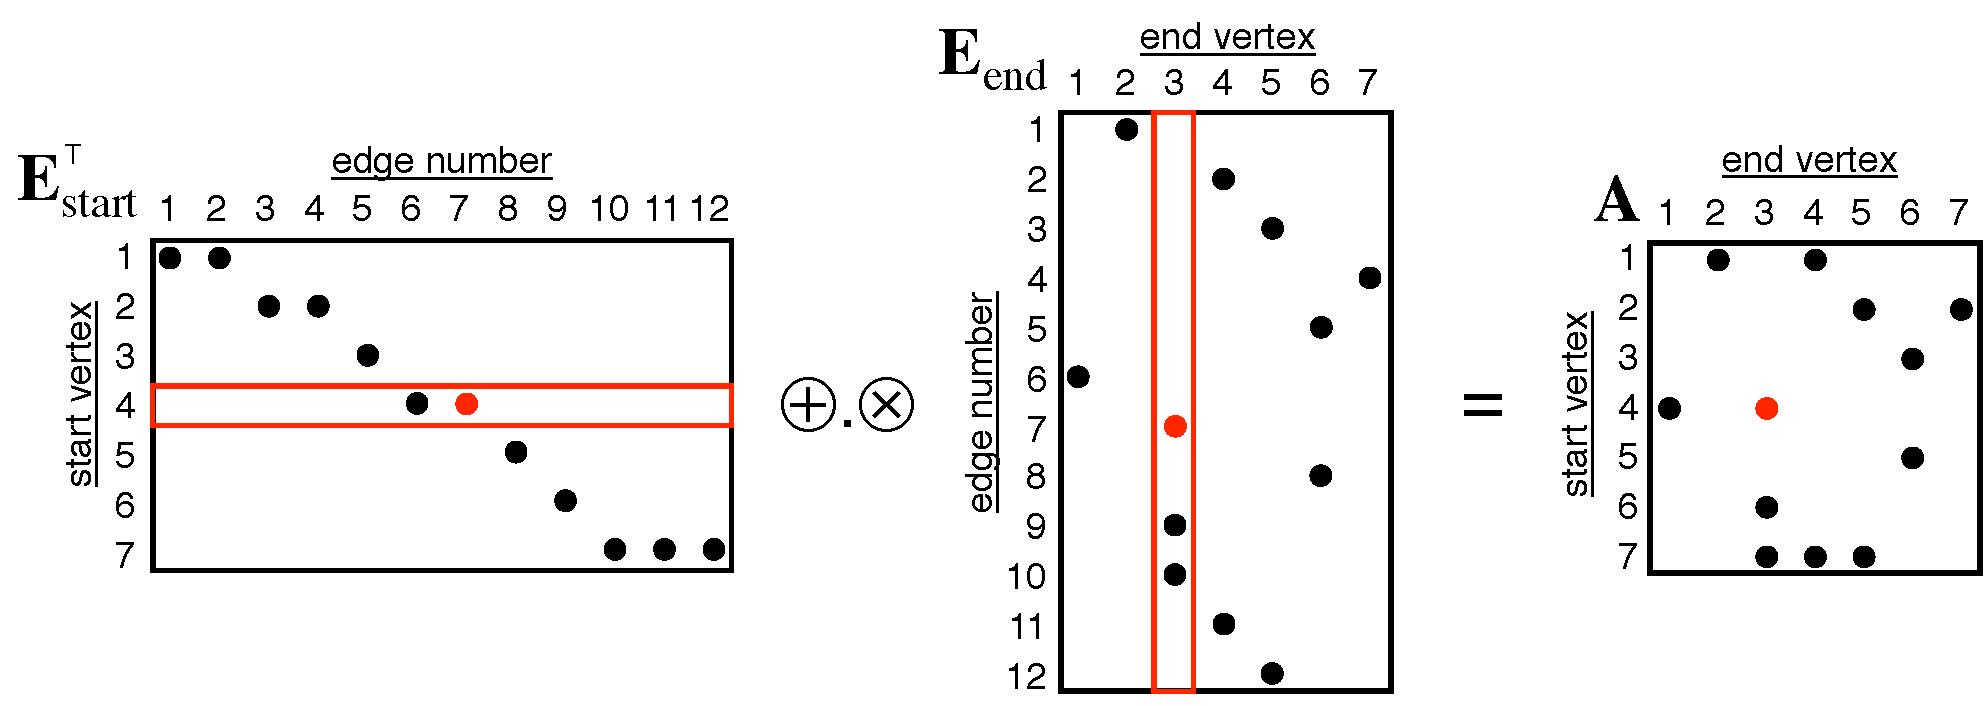
\includegraphics[width=5in]{figures/AdjacencyMatrixToIncidence.pdf}
      \caption{Construction of an adjacency matrix of a graph from its incidence matrices via matrix-matrix multiply.  The entry $\mathbf{A}(4,3)$ is obtained by combining the row vector $\mathbf{E}_\mathrm{start}^{\sf T}(4,k)$ with the column vector $\mathbf{E}_\mathrm{end}(k,3)$ via matrix-matrix product $\mathbf{A}(4,3)= \bigoplus\limits_{k = 1}^{13} \mathbf{E}_\mathrm{start}^{\sf T}(4,k) \otimes \mathbf{E}_\mathrm{end}(k,3)$}
      \label{fig:AdjacencyToIncidence}
\end{figure}


\subsection{accumulation: Summing up Edge Weights}

{\bf mxm} can be used to multiply and accumulate values into a matrix.  One example is when the result of multiply ${\bf A}$ and ${\bf B}$ is added to the existing values in ${\bf C}$ (instead of replacing ${\bf C}$.  This can be written
$$
   {\bf C} ~~ {+}{=} ~~ {\bf A} {\bf B}
$$
or more explicitly
$$
   {\bf C}(i,j) = {\bf C}(i,j) + \sum_{k=1}^M {\bf A}(i,k) {\bf B}(k,j)
$$

\subsection{transposing Inputs or Outputs: Swapping Start and End Vertices}

Another variant is to specify that the matrix multiply should be performed over the transpose of  ${\bf A}$, ${\bf B}$, or ${\bf C}$.

Transposing the input matrix ${\bf A}$ implies
$$
   {\bf C} = {\bf A}^{\sf T} {\bf B}
$$
or more explicitly
$$
   {\bf C}(i,j) = \sum_{k=1}^n {\bf A}(k,i) {\bf B}(k,j)
$$
where ${\bf A}: \mathbb{R}^{n \times m}$.

Transposing the input matrix ${\bf B}$ implies
$$
   {\bf C} = {\bf A} {\bf B}^{\sf T}
$$
or more explicitly
$$
   {\bf C}(i,j) = \sum_{k=1}^l {\bf A}(i,k) {\bf B}(j,k)
$$
where ${\bf B}: \mathbb{R}^{l \times n}$.


Transposing the output matrix ${\bf C}$ implies
$$
   {\bf C}^{\sf T} = {\bf A} {\bf B}
$$
or more explicitly
$$
   {\bf C}(j,i) = \sum_{k=1}^l {\bf A}(i,k) {\bf B}(k,j)
$$
where ${\bf C}: \mathbb{R}^{m \times n}$.

Other combinations include transposing both inputs ${\bf A}$ and ${\bf B}$
$$
   {\bf C} = {\bf A}^{\sf T} {\bf B}^{\sf T} ~~~~~~~~ \Rightarrow ~~~~~~~~ {\bf C}(i,j) = \sum_{k=1}^M {\bf A}(k,i) {\bf B}(j,k)
$$
where ${\bf A}: \mathbb{R}^{l \times m}$ and ${\bf B}: \mathbb{R}^{n \times l}$; transposing both input ${\bf A}$ and output ${\bf C}$
$$
   {\bf C}^{\sf T} = {\bf A}^{\sf T} {\bf B} ~~~~~~~~ \Rightarrow ~~~~~~~~ {\bf C}(j,i) = \sum_{k=1}^l {\bf A}(k,i) {\bf B}(k,j)
$$
where ${\bf A}: \mathbb{R}^{l \times m}$, ${\bf B}: \mathbb{R}^{l \times n}$, and ${\bf C}: \mathbb{R}^{m \times n}$; and transposing both input ${\bf B}$ and output ${\bf C}$
$$
   {\bf C}^{\sf T} = {\bf A} {\bf B}^{\sf T} ~~~~~~~~ \Rightarrow ~~~~~~~~ {\bf C}(j,i) = \sum_{k=1}^l {\bf A}(i,k) {\bf B}(j,k)
$$
where ${\bf A}: \mathbb{R}^{m \times l}$, ${\bf B}: \mathbb{R}^{n \times l}$ and ${\bf C}: \mathbb{R}^{n \times m}$.

Normally, the transpose operation distributes over matrix multiplication
$$
({\bf A} {\bf B})^{\sf T} ={\bf B}^{\sf T} {\bf A}^{\sf T}
$$
and so transposing both inputs ${\bf A}$ and ${\bf B}$ and the output ${\bf C}$ is rarely used.  Nevertheless, for completeness, this operation is defined as
$$
   {\bf C}^{\sf T} = {\bf A}^{\sf T} {\bf B}^{\sf T} ~~~~~~~~ \Rightarrow ~~~~~~~~ {\bf C}(j,i) = \sum_{k=1}^l {\bf A}(k,i) {\bf B}(j,k)
$$
where ${\bf A}: \mathbb{R}^{l \times m}$, ${\bf B}: \mathbb{R}^{n \times l}$, and ${\bf C}: \mathbb{R}^{n \times m}$.

\subsection{addition and multiplication: Combining and Scaling Edges}
  Standard matrix multiplication on real numbers first performs scalar arithmetic multiplication on the elements and then performs scalar arithmetic addition on the results.  The GraphBLAS allows the scalar operations of addition $\oplus$ and multiplication $\otimes$ to be replaced with user defined functions.  This can be formally denoted as
$$
   {\bf C} = {\bf A} ~ {\oplus}.{\otimes} ~ {\bf B}
$$
or more explicitly
$$
   {\bf C}(i,j) = \bigoplus_{k=1}^l {\bf A}(i,k) \otimes {\bf B}(k,j)
$$
where ${\bf A}: \mathbb{S}^{m \times l}$,  ${\bf B}: \mathbb{S}^{m \times l}$, and ${\bf C}: \mathbb{S}^{m \times n}$.  In this notation, standard matrix multiply can be written
$$
   {\bf C} = {\bf A} ~ {+}.{\times} ~ {\bf B}
$$
where $\mathbb{S} \rightarrow \mathbb{R}$. Other matrix multiplications of interest include max-plus algebras
$$
   {\bf C} = {\bf A} ~ {\max}.{+} ~ {\bf B}
$$
or more explicitly
$$
   {\bf C}(i,j) = \max_k \{{\bf A}(i,k) + {\bf B}(k,j)\}
$$
where $\mathbb{S} \rightarrow \{-\infty \cup \mathbb{R}\}$; min-max algebras
$$
   {\bf C} = {\bf A} ~ {\min}.{\max} ~ {\bf B}
$$
or more explicitly
$$
   {\bf C}(i,j) = \min_k \{\max({\bf A}(i,k),{\bf B}(k,j))\}
$$
where $\mathbb{S} \rightarrow [0,\infty)$; the Galois field of order 2
$$
   {\bf C} = {\bf A} ~ {\rm xor}.{\rm and} ~ {\bf B}
$$
or more explicitly
$$
   {\bf C}(i,j) = {\rm xor}_k \{\rm and({\bf A}(i,k),{\bf B}(k,j))\}
$$
where $\mathbb{S} \rightarrow [0,1]$; and power set algebras
$$
   {\bf C} = {\bf A} ~ {\cup}.{\cap} ~ {\bf B}
$$
or more explicitly
$$
   {\bf C}(i,j) = \bigcup_{k=1}^M {\bf A}(i,k) \cap {\bf B}(k,j)
$$
where $\mathbb{S} \rightarrow \{\mathbb{Z}\}$.

  Accumulation also works with user defined addition and can be denoted
$$
   {\bf C} ~~ {\oplus}{=} ~~ {\bf A} ~ {\oplus}.{\otimes} ~ {\bf B}
$$
or more explicitly
$$
   {\bf C}(i,j) = {\bf C}(i,j) \oplus \bigoplus_{k=1}^M {\bf A}(i,k) \otimes {\bf B}(k,j)
$$

\section{mxv}
  Using notation similar to {\bf mxm}, matrix vector multiply can be represented by the following mathematical statement
$$
   {\bf c} ~~ {\textcolor{blue}{\oplus}}{=} ~~ {\bf A}^{\textcolor{blue}{\sf T}} ~ {\oplus}.{\otimes} ~ {\bf b}
$$
where  ${\bf A}: \mathbb{S}^{m \times n}$,  ${\bf b}: \mathbb{S}^{n}$, and ${\bf c}: \mathbb{S}^{m}$

\section{vxm}
  Using notation similar to {\bf mxm},  vector matrix multiply can be represented by the following mathematical statement
$$
   {\bf c} ~~ {\textcolor{blue}{\oplus}}{=} ~~ {\bf a} ~ {\oplus}.{\otimes} ~ {\bf B}^{\textcolor{blue}{\sf T}}
$$
where  ${\bf a}: \mathbb{S}^{m}$, ${\bf B}: \mathbb{S}^{m \times n}$, and ${\bf c}: \mathbb{S}^{n}$

\section{extract: Selecting Sub-Graphs}
  Selecting sub-graphs is a very common graph operation (see Figure~\ref{fig:AdjacencyMatrixSub}).  The GraphBLAS performs this operation with the {\bf Extract} function by selecting starting vertices (row) and ending vertices (columns) from a matrix $\mathbf{A} : \mathbb{S}^{m \times n}$
$$
   \mathbf{C}^{\textcolor{blue}{\sf T}} ~~ {\textcolor{blue}{\oplus}}{=} ~~  \mathbf{A}^{\textcolor{blue}{\sf T}}({\bf i},{\bf j})
$$
or more explicitly
$$
   {\bf C}(i,j) = {\bf A}({\bf i}(i),{\bf j}(j))
$$
where $i \in \{1,...,m_C\}$, $j \in \{1,...,n_C\}$, ${\bf i} : I^{m_C}$, and ${\bf j}: J^{n_C}$  select specific sets of rows and columns in a specific order.   The resulting matrix $\mathbf{C} : \mathbb{S}^{m_C \times n_C}$ can be larger or smaller than the input matrix $\mathbf{A}$.  {\bf Extract} can also be used to replicate and/or permute rows and columns in a matrix.

  {\bf extract} can be implemented using sparse matrix multiply as
$$
   \mathbf{C}= \mathbf{S}({\bf i}) ~ \mathbf{A} ~ \mathbf{S}^{\sf T}({\bf j})
$$
where $\mathbf{S}({\bf i})$ and $\mathbf{S}({\bf j})$ are selection matrices given by
$$
   \mathbf{S}({\bf i}) = \mathbb{S}^{m_C \times m}(\{1,...,m_C\},{\bf i},1)
$$
$$
    \mathbf{S}({\bf j}) = \mathbb{S}^{n_C \times n}(\{1,...,n_C\},{\bf j},1)
$$

\begin{figure}[!htb]
  \centering
    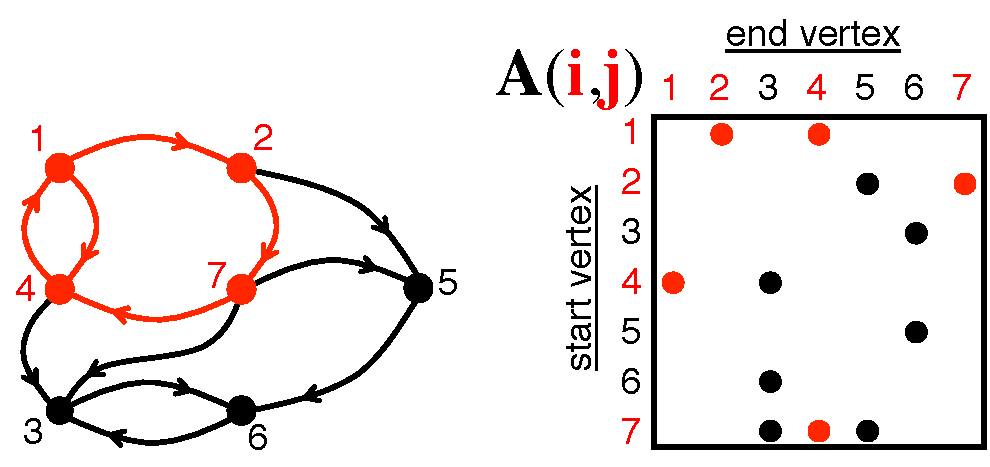
\includegraphics[width=3in]{figures/AdjacencyMatrixSub.pdf}
      \caption{Selection of a 4 vertex sub-graph from the adjacency matrix via selecting sub-sets of rows and columns ${\bf i} = {\bf j} = \{1,2,4,7\}$.}
      \label{fig:AdjacencyMatrixSub}
\end{figure}

\section{assign: Modifying Sub-Graphs}
  Modifying sub-graphs is a very common graph operation.  The GraphBLAS performs this operation with the {\bf Assign} function by selecting starting vertices (row) and ending vertices (columns) from a matrix $\mathbf{C} : \mathbb{S}^{m \times n}$ and assigning new values to them from another sparse matrix, $\mathbf{A} : \mathbb{S}^{m_A \times n_A}$
$$
   \mathbf{C}^{\textcolor{blue}{\sf T}}({\bf i},{\bf j}) ~~ {\textcolor{blue}{\oplus}}{=} ~~ \mathbf{A}^{\textcolor{blue}{\sf T}}
$$
or more explicitly
$$
   {\bf C}({\bf i}(i),{\bf j}(j)) ~~ {\textcolor{blue}{\oplus}}{=} ~~{\bf A}(i,j) 
$$
where $i \in \{1,...,m_A\}$, $j \in \{1,...,n_A\}$, ${\bf i} : I^{m_A}$ and ${\bf j}: J^{n_A}$ select specific sets of rows and columns in a specific order and ${\textcolor{blue}{\oplus}}$ optionally allows $\mathbf{A}$ to added to the existing values of $\mathbf{C}$. 

  The additive form of {\bf Extract} can be implemented using sparse matrix multiply as
$$
   \mathbf{C} ~~ {\oplus}{=} ~~ \mathbf{S}^{\sf T}({\bf i}) ~ \mathbf{A} ~ \mathbf{S}({\bf j})
$$
where $\mathbf{S}({\bf i})$ and $\mathbf{S}({\bf j})$ are selection matrices given by
$$
   \mathbf{S}({\bf i}) = \mathbb{S}^{m_A \times m}(\{1,...,m_A\},{\bf i},1)
$$
$$
    \mathbf{S}({\bf j}) = \mathbb{S}^{n_A \times n}(\{1,...,n_A\},{\bf j},1)
$$
  

\section{eWiseAdd, eWiseMult: Combining Graphs, Intersecting Graphs, Scaling Graphs}
  Combining graphs along with adding their edge weights can be accomplished by adding together their sparse matrix representations. {\bf EwiseAdd} provides this operation
$$
   {\bf C}^{\textcolor{blue}{\sf T}} ~~ {\textcolor{blue}{\oplus}}{=} ~~ {\bf A}^{\textcolor{blue}{\sf T}} ~~ \oplus ~~ {\bf B}^{\textcolor{blue}{\sf T}}
$$
where ${\bf A},{\bf B},{\bf C}: \mathbb{S}^{m \times n}$ or more explicitly 
$$
   {\bf C}(i,j) ~~ = ~~ {\bf C}(i,j) ~~ {\textcolor{blue}{\oplus}} ~~ {\bf A}(i,j) ~~ \oplus ~~{\bf B}(i,j)
$$
where $i \in \{1,...,m\}$, and $j \in \{1,...,n\}$ and ${\textcolor{blue}{\oplus}}$ is an optional argument. 

  Intersecting graphs along with scaling their edge weights can be accomplished by element-wise multiplication of their sparse matrix representations. {\bf EwiseMult} provides this operation
$$
   {\bf C}^{\textcolor{blue}{\sf T}} ~~ {\textcolor{blue}{\oplus}}{=} ~~ {\bf A}^{\textcolor{blue}{\sf T}} ~~ \otimes ~~ {\bf B}^{\textcolor{blue}{\sf T}}
$$
where ${\bf A},{\bf B},{\bf C}: \mathbb{S}^{m \times n}$ or more explicitly 
$$
   {\bf C}(i,j) ~~ = {\bf C}(i,j) ~~ {\textcolor{blue}{\oplus}} ~~ {\bf A}(i,j) ~~ \otimes ~~{\bf B}(i,j)
$$
where $i \in \{1,...,m\}$, and $j \in \{1,...,n\}$ and ${\textcolor{blue}{\oplus}}$ is an optional argument. 

\section{apply: Modify Edge Weights}
  Modifying edge weights can be done by via the element-wise by unary function $f()$ to the values of a sparse matrix
$$
   {\bf C} ~~ {\textcolor{blue}{\oplus}}{=} ~~ f({\bf A})
$$
or more explicitly
$$
   {\bf C}(i,j) = {\textcolor{blue}{\bf C}}(i,j) ~ {\textcolor{blue}{\oplus}} ~f({\bf A}(i,j))
$$
where ${\bf A},{\bf C}: \mathbb{S}^{m \times n}$, and $f(0) = 0$.

  {\bf Apply} can be implemented via {\bf EwiseMult} via
$$
   {\bf C} ~~ {\textcolor{blue}{\oplus}}{=} ~~ {\bf A} \otimes {\bf A}
$$
where $\otimes \equiv f()$ and $f(a,a) = f(a)$.

\section{reduce: Compute Vertex Degrees}
  It is often desired to combine the weights of all the vertices that come out of the same starting vertices.  This aggregation can be represented as a matrix product as
$$
   {\bf c} ~~ {\textcolor{blue}{\oplus}}{=} {\bf A} ~~ {\oplus}.{\otimes} ~~{\bf 1}
$$
or more explicitly
$$
   {\bf c}(i,1) = {\textcolor{blue}{\bf c}}(i,1) ~~ {\textcolor{blue}{\oplus}} ~~ \bigoplus_{j=1}^M {\bf A}(i,j)
$$
where ${\bf c}: \mathbb{S}^{m \times 1}$ and ${\bf A}: \mathbb{S}^{m \times n}$, and ${\bf 1}: \mathbb{S}^{n \times 1}$ is a column vector of all ones.

Likewise, combining all the weights of all the vertices that go into the same ending vertices can be represented as matrix product as
$$
   {\bf c} ~~ {\textcolor{blue}{\oplus}}{=}  {\bf 1} ~~ {\oplus}.{\otimes} ~~{\bf A} 
$$
or more explicitly
$$
   {\bf c}(1,j) = {\textcolor{blue}{\bf c}}(1,j) ~~ {\textcolor{blue}{\oplus}} ~~ \bigoplus_{i=1}^m {\bf A}(i,j)
$$
where ${\bf c}: \mathbb{S}^{1 \times n}$ and ${\bf A}: \mathbb{S}^{m \times n}$, and ${\bf 1}: \mathbb{S}^{1 \times m}$ is a row vector of all ones.


\section{Kronecker: Graph Generation (Proposal)}

  Generating graphs is a common operation in a wide range of graph algorithms.  Graph generation is used in testing graphs algorithms, creating graph templates to match against, and to compare real graph data with models.  The Kronecker product of two matrices is a convenient and well-defined matrix operation that can be used for generating a wide range of graphs from a few a parameters.

The Kronecker product is defined as follows
  $$
    {\bf C} = {\bf A} ~ \text{\footnotesize \textcircled{\raisebox{-0.3pt}{\footnotesize $\otimes$}}} ~ {\bf B} = \left(
     \begin{array}{cccc}
        {\bf A}(1,1) \otimes {\bf B} & {\bf A}(1,2) \otimes {\bf B} & ... & {\bf A}(1,n_A) \otimes {\bf B} \\
        {\bf A}(2,1) \otimes {\bf B} & {\bf A}(2,2) \otimes {\bf B} & ... & {\bf A}(2,n_A) \otimes {\bf B} \\
         \vdots   &  \vdots   &     & \vdots \\
        {\bf A}(m_A,1) \otimes {\bf B} & {\bf A}(m_A,2) \otimes {\bf B} & ... & {\bf A}(m_A,n_A) \otimes {\bf B} \\
     \end{array}  \right)
  $$
where ${\bf A} : {\mathbb S}^{m_A \times n_A}$, ${\bf B} : {\mathbb S}^{m_B \times n_B}$, and
${\bf C} : {\mathbb S}^{m_A m_B \times n_A n_B}$.  More explicitly, the Kronecker product can be written as
  $$
    {\bf C}((i_A-1) m_A + i_B,(j_A-1) n_A + j_B) = {\bf A}(i_A,j_A) \otimes {\bf B}(i_B,j_B)
  $$
With the usual accumulation and transpose options, the Kronecker product can be written
  $$
    {\bf C}^{\textcolor{blue}{\sf T}} ~~ {\textcolor{blue}{\oplus}}{=} {\bf A}^{\textcolor{blue}{\sf T}} ~ \text{\footnotesize \textcircled{\raisebox{-0.3pt}{\footnotesize $\otimes$}}} ~ {\bf B}^{\textcolor{blue}{\sf T}}
  $$
The elements-wise multiply operation $\otimes$ can be user defined so long as the resulting operation obeys the aforementioned rules on elements-wise multiplication such as the multiplicative annihilator.  If  elements-wise multiplication and addition obey the conditions specified in section 2.5, then the Kronecker product has many of the same desirable properties, such as associativity
  $$
    ({\bf A} ~ \text{\footnotesize \textcircled{\raisebox{-0.3pt}{\footnotesize $\otimes$}}} ~ {\bf B}) ~ \text{\footnotesize \textcircled{\raisebox{-0.3pt}{\footnotesize $\otimes$}}} ~ {\bf C} = 
    {\bf A} ~ \text{\footnotesize \textcircled{\raisebox{-0.3pt}{\footnotesize $\otimes$}}} ~ ({\bf B} ~ \text{\footnotesize \textcircled{\raisebox{-0.3pt}{\footnotesize $\otimes$}}} ~ {\bf C})
  $$
and element-wise distributivity over addition
 $$
    {\bf A} ~ \text{\footnotesize \textcircled{\raisebox{-0.3pt}{\footnotesize $\otimes$}}} ~ ({\bf B} \oplus {\bf C}) = 
    ({\bf A} ~ \text{\footnotesize \textcircled{\raisebox{-0.3pt}{\footnotesize $\otimes$}}} ~ {\bf B}) \oplus ~ ({\bf A} ~ \text{\footnotesize \textcircled{\raisebox{-0.3pt}{\footnotesize $\otimes$}}} ~ {\bf C})
  $$
Finally, one unique feature of the Kronecker product is its relation to the matrix product
  $$
    ({\bf A} ~ \text{\footnotesize \textcircled{\raisebox{-0.3pt}{\footnotesize $\otimes$}}} ~ {\bf B}) ({\bf C} ~ \text{\footnotesize \textcircled{\raisebox{-0.3pt}{\footnotesize $\otimes$}}} ~ {\bf D})
     = 
     ({\bf A} {\bf C}) ~ \text{\footnotesize \textcircled{\raisebox{-0.3pt}{\footnotesize $\otimes$}}} ~ ({\bf B} {\bf D})
   $$

\section{Graph Algorithms and Diverse Semirings}

   The ability to change $\oplus$ and $\otimes$ operations allows different graph algorithms to be implemented using the same element-wise addition, element-wise multiplication, and matrix multiplication operations.  Different semirings are best suited for certain classes of graph algorithms.  The  pattern of non-zero entries resulting from breadth-first-search  illustrated in Figure~\ref{fig:AdjacencyMatrixBFS} is generally preserved for various semirings.  However, the non-zero values assigned to the edges and vertices can be very different and enable different graph algorithms.
   
   \begin{figure}[!htb]
  \centering
    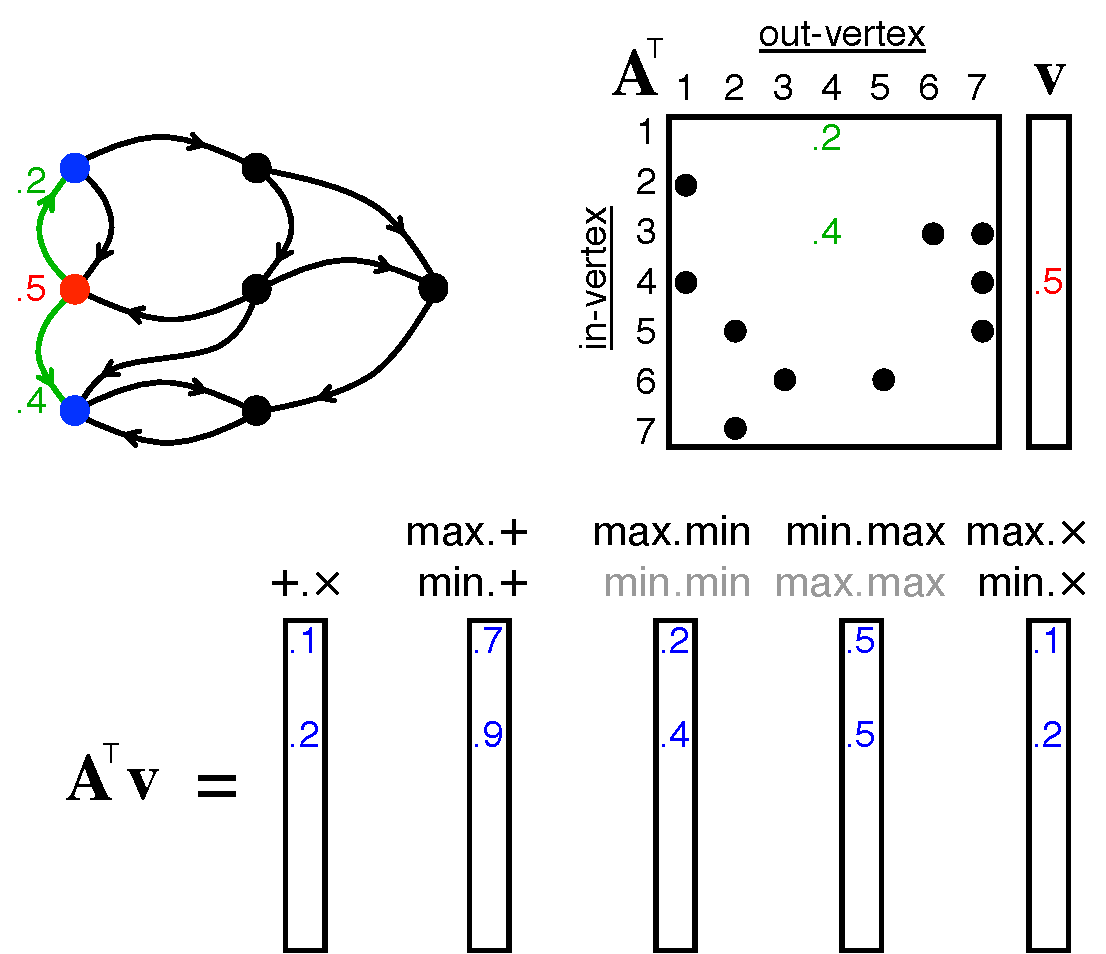
\includegraphics[width=4in]{figures/AdjacencyMatrixSemiring1hop.pdf}
      \caption{(top left) One-hop breadth-first-search of a weighted graph starting at vertex 4 and traversing to vertices 1 and 3.  (top right) Matrix representation of the weighted graph and vector representation of the starting vertex.  (bottom) Matrix-vector multiplication of the adjacency matrix of a graph performs the equivalent operation.  Different pairs of operations $\oplus$ and $\otimes$ produce different results. For display convenience, operator pairs that produce the same values \emph{in this specific example} are stacked.}
      \label{fig:AdjacencyMatrixSemiring1hop}
\end{figure}

\begin{figure}[!htb]
  \centering
    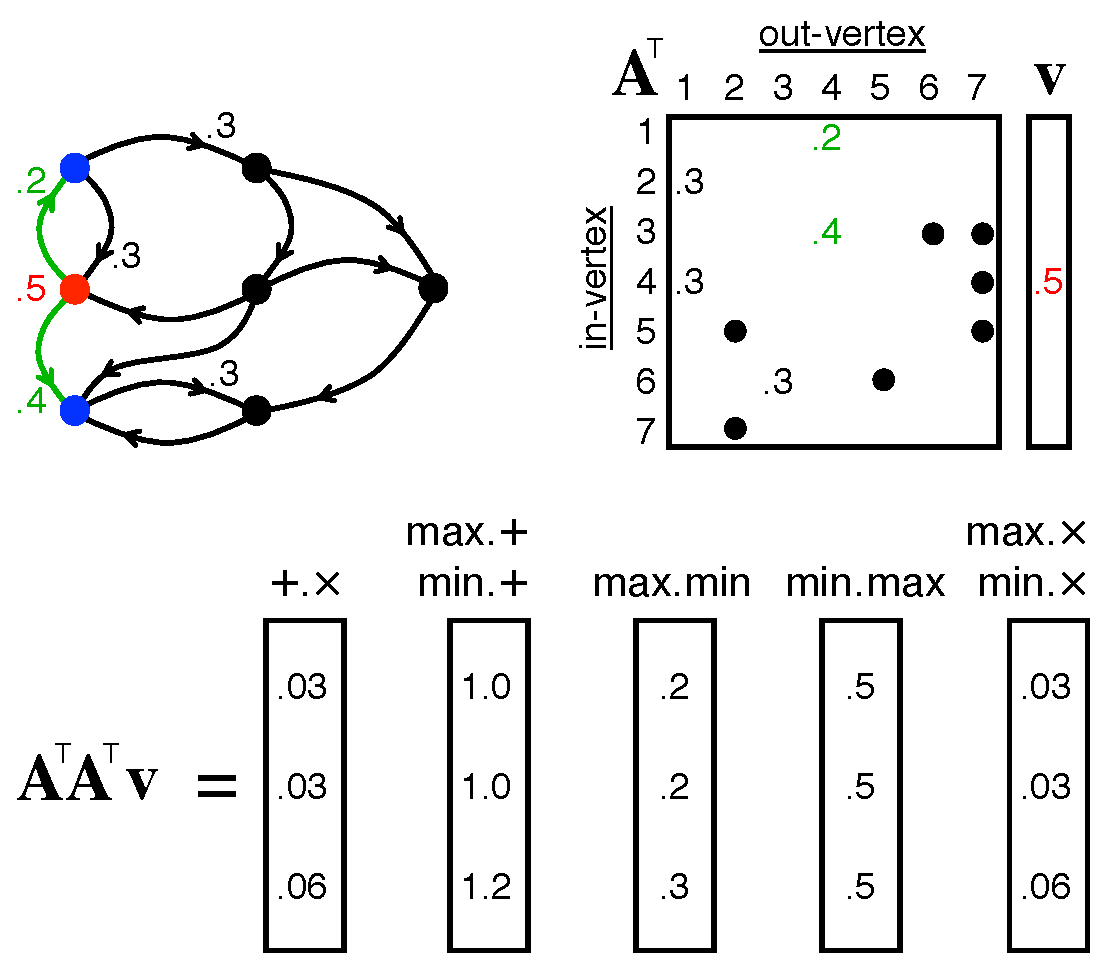
\includegraphics[width=4in]{figures/AdjacencyMatrixSemiring2hop.pdf}
      \caption{(top left) Two-hop breadth-first-search of a weighted graph starting at vertex 4 and traversing to vertices 1 and 3 and continues on to vertices 2, 4, and 6. (top right) Matrix representation of the weighted graph and vector representation of the starting vertex. (bottom) Matrix-vector multiplication of the adjacency matrix of a graph performs the equivalent operation.  Different pairs of operations $\oplus$ and $\otimes$ produce different results. For display convenience, operator pairs that produce the same result \emph{in this specific example} are stacked.
%Semiring operators pairs are shown in black and non-semiring operator pairs are shown in grey.
}
      \label{fig:AdjacencyMatrixSemiring2hop}
\end{figure}

  Figure~\ref{fig:AdjacencyMatrixSemiring1hop} illustrates performing a single-hop breadth-first-search using seven semirings (${+}.{\times}$, ${\max}.{+}$, ${\min}.{+}$, ${\max}.{\min}$, ${\min}.{\max}$, ${\max}.{\times}$, and ${\min}.{\times}$).
%and two non-semirings (${\min}.{\min}$ and ${\max}.{\max}$).
For display convenience, operator pairs that produce the same result \emph{in this specific example} are stacked.  In Figure~\ref{fig:AdjacencyMatrixSemiring1hop} the starting vertex 4 is assigned a value of .5 and the edges to its vertex neighbors 1 and 3 are assigned values of .2 and .4.  Empty values are assumed to be the corresponding 0 of the operator pair. In all cases, the pattern of non-zero entries of the results are the same.  In each case, because there is only one path from vertex 4 to vertex 1 and from vertex 4 to vertex 3, the only effect of the $\otimes$ of operator is to compare the non-zero output the $\otimes$ operator with the 0.  Thus, the differences between the $\oplus$ operators have no impact in this specific example because for any values of $a$
$$
  a \oplus 0 = 0 \oplus a = a
$$

  The graph algorithm implications of different ${\oplus}.{\otimes}$ operator pairs is more clearly seen in the two-hop breadth-first-search.  Figure~\ref{fig:AdjacencyMatrixSemiring2hop} illustrates graph traversal that starts at vertex 4, goes to vertices 1 and 3, and then continues on to vertices 2, 4, and 6. For simplicity, the additional edge weights are assigned values of .3.  The first operator pair ${+}.{\times}$ provides the product of all the weights of all paths from the starting vertex to each ending vertex.  The ${+}.{\times}$ semiring is valuable for determining the strengths of all the paths between the starting and ending vertices.  In this example,  there is only one path between the starting vertex and the ending vertices and so ${+}.{\times}$ and ${\max}.{\times}$ and ${\min}.{\times}$ all produce the same results.  If there were multiple paths between the start and end vertices then $\oplus$ would operate on more than one non-zero value and the differences would be apparent.  Specifically, ${+}.{\times}$ combines all paths while ${\max}.{\times}$ and ${\min}.{\times}$ selects either the minimum or the maximum path.  Thus, these different operator pairs represent  different graph algorithms.  One algorithm produces a value that combines all paths while the other algorithm produces a value that is derived from a single path.

   A similar pattern can be seen among the other operator pairs.   ${\max}.{+}$ and ${\min}.{+}$ compute the sum of the weights along each path from the starting vertex to each ending vertex and then selects the largest (or smallest) weighted path.  ${\max}.{\min}$ and ${\min}.{\max}$ compute the minimum (or maximum) of the weights along each path from the starting vertex to each end vertex and then selects the largest (or smallest) weighted path.
%${\max}.{\max}$ and ${\min}.{\min}$ compute the minimum (or maximum) of the weights along each path from the starting vertex to each ending vertex and then selects the smallest (or largest) weighted path.
   
  A wide range of breadth-first-search weight computations can be performed via matrix multiplication with different operator pairs.  A synopsis of the types of calculations illustrated in Figures~\ref{fig:AdjacencyMatrixSemiring1hop} and \ref{fig:AdjacencyMatrixSemiring2hop} is as follows
\begin{description}
\item[${+}.{\times}$] sum of products of weights along each path; computes the strength of all connections between the starting vertex and the ending vertices.
\item[${\max}.{\times}$] maximum of products of weights along each path; computes the longest product of all of the connections between the starting vertex and the ending vertices.
\item[${\min}.{\times}$] minimum of products of weights along each path; computes the shortest product of all of the connections between the starting vertex and the ending vertices.
\item[${\max}.{+}$] maximum of sum of weights along each path; computes the longest sum of all of the connections between the starting vertex and the ending vertices.
\item[${\min}.{+}$] minimum of sum of weights along each path; computes the shortest sum of all of the connections between the starting vertex and the ending vertices.
\item[${\max}.{\min}$] maximum of minimum of weight along each path; computes the longest of all the shortest connections between the starting vertex and the ending vertices.
\item[${\min}.{\max}$] minimum of maximum of weight along each path; computes the shortest of all the longest connections between the starting vertex and the ending vertices.
%\item[${\max}.{\max}$] maximum of maximum of weight along each path (not a semiring); computes the longest of all the longest connections between the starting vertex and the ending vertices.
%\item[${\min}.{\min}$] minimum of minimum of weight along each path (not a semiring); computes the shortest of all the shortest connections between the starting vertex and the ending vertices.
\end{description}

%\section{Appendix: Glossary}
%  [Will eventually be moved to front matter.]
%
%\section{Appendix: Examples}
%  [Will eventually be moved to back matter.]
%
%
%For my own reference, I'm leaving in a few latex fragments I'd like to remember for when we add our own text.
%
%
%\begin{boxedcode}
%\#pragma\plc{ }omp\plc{ directive-name [clause[ [},\plc{] clause] ... ] new-line}
%\end{boxedcode}
%
%As an example of how a construct might look, here is the single construct from OpenMP
%
%\subsection{\code{single} Construct}
%\index{single@{\code{single}}}
%\index{constructs!single@{\code{single}}}
%\label{subsec:single Construct}
%\summary
%The \code{single} construct specifies that the associated structured block is executed by only 
%one of the threads in the team (not necessarily the master thread), in the context of its 
%implicit task. The other threads in the team, which do not execute the block, wait at an 
%implicit barrier at the end of the \code{single} construct unless a \code{nowait} clause is specified.
%
%\parbox{\linewidth}{%
%\syntax
%\ccppspecificstart}
%The syntax of the single construct is as follows:
%
%\begin{boxedcode}
%\#pragma omp single \plc{[clause[ [},\plc{] clause] ... ] new-line}
%   \plc{structured-block}
%\end{boxedcode}
%
%\begin{samepage}
%where \plc{clause} is one of the following:
%
%\begin{indentedcodelist}
%private(\plc{list})
%firstprivate(\plc{list})
%copyprivate(\plc{list})
%nowait
%\end{indentedcodelist}
%\ccppspecificend
%\end{samepage}
%
%\fortranspecificstart
%The syntax of the \code{single} construct is as follows:
%
%\begin{boxedcode}
%!\$omp single \plc{[clause[ [},\plc{] clause] ... ]}
%   \plc{structured-block} 
%!\$omp end single \plc{[end\_clause[ [},\plc{] end\_clause] ... ]}
%\end{boxedcode}
%
%where \plc{clause} is one of the following:
%
%\begin{indentedcodelist}
%private(\plc{list})
%firstprivate(\plc{list})
%\end{indentedcodelist}
%
%and \plc{end\_clause} is one of the following: 
%
%\begin{indentedcodelist}
%copyprivate(\plc{list})
%nowait
%\end{indentedcodelist}
%\fortranspecificend
%
%\binding
%The binding thread set for a \code{single} region is the current team. A \code{single} region 
%binds to the innermost enclosing \code{parallel} region. Only the threads of the team 
%executing the binding \code{parallel} region participate in the execution of the structured 
%block and the implied barrier of the \code{single} region if the barrier is not eliminated by a 
%\code{nowait} clause.
%
%\descr
%The method of choosing a thread to execute the structured block is implementation 
%defined. There is an implicit barrier at the end of the \code{single} construct unless a 
%\code{nowait} clause is specified. 
%
%\restrictions
%Restrictions to the \code{single} construct are as follows: 
%
%\begin{itemize}
%\item The \code{copyprivate} clause must not be used with the \code{nowait} clause.
%
%\item At most one \code{nowait} clause can appear on a \code{single} construct.
%
%\cppspecificstart
%\item A throw executed inside a \code{single} region must cause execution to resume within the 
%same \code{single} region, and the same thread that threw the exception must catch it.
%\cppspecificend
%\end{itemize}
%
%
%\crossreferences
%\begin{itemize}
%\item \code{private} and \code{firstprivate} clauses, see 
%\specref{subsec:Data-Sharing Attribute Clauses}.
%
%\item \code{copyprivate} clause, see 
%\specref{subsubsec:copyprivate clause}.
%\end{itemize}
%

% This is the end of ch2-functions.tex of the GraphBLAS specification.

